\documentclass[lettersize,journal]{IEEEtran}
\usepackage{amsmath,amsfonts}
\usepackage{algorithmic}
\usepackage{algorithm}
\usepackage{array}
%\usepackage{minted}
\usepackage[caption=false,font=normalsize,labelfont=sf,textfont=sf]{subfig}
\usepackage{textcomp}
\usepackage{lipsum}
\usepackage{xcolor}
\usepackage[export]{adjustbox}
\usepackage{stfloats}
\usepackage{url}
\usepackage{verbatim}
\usepackage{graphicx}
\usepackage{cite}
\usepackage[hidelinks]{hyperref}
\usepackage{enumitem}
\usepackage{listings}
\usepackage{booktabs}
\usepackage{caption}
\hyphenation{op-tical net-works semi-conduc-tor IEEE-Xplore} % todo remove
% updated with editorial comments 8/9/2021
\usepackage{utfsym}
\usepackage{makecell}
\renewcommand{\checkmark}{\usym{1F5F8}}
\newcommand{\cfgfiles}{configuration files}
\newcommand{\cfgfile}{configuration file}
\newcommand{\toolname}{\textit{MetaConfigurator}}
\newcommand{\jskeyword}[1]{\texttt{#1}} % use for json schema keywords

\colorlet{punct}{red!60!black}
\definecolor{background}{HTML}{EEEEEE}
\definecolor{delim}{RGB}{20,105,176}
\colorlet{numb}{magenta!60!black}

% adding code style for json
\lstdefinelanguage{json}{
 basicstyle=\small\ttfamily,
 numbers=left,
 xleftmargin=2.0ex,
 float=htb,
 numberstyle=\scriptsize,
 stepnumber=1,
 numbersep=8pt,
 showstringspaces=false,
 breaklines=true,
 frame=lines,
 backgroundcolor=\color{background},
 literate=
 *{0}{{{\color{numb}0}}}{1}
  {1}{{{\color{numb}1}}}{1}
  {2}{{{\color{numb}2}}}{1}
  {3}{{{\color{numb}3}}}{1}
  {4}{{{\color{numb}4}}}{1}
  {5}{{{\color{numb}5}}}{1}
  {6}{{{\color{numb}6}}}{1}
  {7}{{{\color{numb}7}}}{1}
  {8}{{{\color{numb}8}}}{1}
  {9}{{{\color{numb}9}}}{1}
  {:}{{{\color{punct}{:}}}}{1}
  {,}{{{\color{punct}{,}}}}{1}
  {\{}{{{\color{delim}{\{}}}}{1}
  {\}}{{{\color{delim}{\}}}}}{1}
  {[}{{{\color{delim}{[}}}}{1}
  {]}{{{\color{delim}{]}}}}{1},
  string=[s]{"}{"},
  comment=[l]{:\ "},
  morecomment=[l]{:"},
}

\captionsetup[lstlisting]{font=small, justification=justified, singlelinecheck=false}
\captionsetup[figure]{font=small, justification=justified, singlelinecheck=false}
\captionsetup[table]{font=sc, justification=centering, singlelinecheck=false, labelsep=newline}

\begin{document}

 \title{Design, Implementation, and Evaluation of a Meta Configuration Tool Using a Schema-to-UI Approach}
 \author{Felix Neubauer, Paul Bredl, Minye Xu, Keyuriben Patel}
%\author{IEEE Publication Technology,~\IEEEmembership{Staff,~IEEE,}
 % <-this % stops a space
%\thanks{This paper was produced by the IEEE Publication Technology Group. They are in Piscataway, NJ.}% <-this % stops a space
%\thanks{Manuscript received April 19, 2021; revised August 16, 2021.}}

% The paper headers
 %\markboth{Journal of best software 2023}%
 %{Shell \MakeLowercase{\textit{et al.}}: Revolutionizing Software}

%\IEEEpubid{0000--0000/00\$00.00~\copyright~2021 IEEE}
% Remember, if you use this you must call \IEEEpubidadjcol in the second
% column for its text to clear the IEEEpubid mark.

 \maketitle

 \begin{abstract}
 Textual formats to structure data, such as JSON, XML, and YAML, are widely used for structuring data in various domains, from configuration files to research data.
 However, managing and modifying data in these formats can be complex and time-consuming.
 While graphical user interfaces (GUIs) are effective in simplifying data management, they require substantial development and maintenance efforts.
 To address this challenge, we introduce \toolname: an innovative web application that generates its GUI depending on a given schema.
 Our approach differs from other schema-to-UI approaches in three key ways: 1) It offers a unified view that combines the benefits of both GUIs and code editors,
 2) it enables schema editing within the same tool, and 3) it supports advanced schema features, including conditions and constraints.
 In this paper, we discuss the design and implementation of \toolname, backed by insights from a small-scale qualitative user study.
The results indicate the effectiveness of our approach in retrieving information from data and schemas and in editing them.


 \end{abstract}

 \begin{IEEEkeywords}
  JSON, YAML, configuration, schema, GUI
 \end{IEEEkeywords}


 \section{Introduction}\label{sec:introduction} %felix

 Textual formats to structure data, such as JSON, XML and YAML, are often used for configuration files or to structure measurement
 or research data, since they can be read and maintained by humans, as well as deserialized and used by computer programs.
 The format of data structures can be defined by so-called schemas, which define the rules the data has to conform to.
 Given a schema, it can be validated whether a particular file confirms to that schema.
 For the sake of simplicity, we will call all file instances using such formats \textit{\cfgfiles}.
 Depending on the domain of such \cfgfiles, they can be complex and time-consuming to modify and maintain.
 Tooling, such as graphical user interfaces, can significantly reduce manual efforts and assist the user in editing the files.
 Those graphical user interfaces (GUIs), however, require initial effort to be developed, as well as continuous effort in being maintained and updated when the underlying data schema changes.
 We tackle this problem by developing a web application that automatically generates such assisting GUIs, based on the given data schema.
 Our approach differs from other schema-to-UI approaches in following:

 \begin{enumerate}
  \item The tool combines the assistance of a GUI with the flexibility and speed of a code editor by providing both in one view.
  This code editor is a text editor that assists with typical features, such as syntax highlighting, auto-completion, and error highlighting.
  \item The schema can be edited using the same tool and type of view.
  We use the same technique to generate a GUI using the \textit{meta schema} of the schema language.
  The meta schema is the schema that defines the schema language itself.
  Thus, the user is presented with a similar view for editing the schema as for editing the \cfgfiles{}.
  \item We support more complex schema features, such as conditions and constraints.
 \end{enumerate}


 In section~\ref{sec:research}, we discuss related work and existing schema formats, as well as schema-to-gui approaches.
 In section~\ref{sec:evaluation-of-schema-languages}, we evaluate existing schema languages to find the most suitable one for this work.
 Section~\ref{sec:design} describes the design and introduces the architecture of \toolname{}.
 Next, in section~\ref{sec:implementation}, we cover the implementation of \toolname{}.
 This includes a detailed description of the schema preprocessing steps, which are necessary to support some of the advanced schema features.
 To gather feedback and verify whether the tool can and will be used in the real world, we conducted a user study, which is described in section~\ref{sec:user_study}.
 We discuss the implications of the results in section~\ref{sec:discussion}.
 Finally, we conclude our work in section~\ref{sec:conclusion}.


 \section{Related Work}\label{sec:research}
 % intro: felix

This sections covers existing schema languages and existing approaches to generate UIs from them.
% We compare the schema languages briefly and discuss why JSON schema is the most useful language for our approach.
As our research is of practical nature, we also consider gray literature such as specifications of schemas or websites.
\subsection{Schema Languages}\label{subsec:schemalanguages}

\textit{Schema languages} are formal languages that specify the structure, constraints, and relationships of data, for example in a database or in structured data formats.

As this work is concerned with generating a GUI based on a schema, we need to choose a suitable schema language.
The following sections describe existing schema languages.
In section \ref{sec:evaluation-of-schema-languages}, we will evaluate which schema language is most suitable for this work.

%paul
\subsubsection{JSON schema}

JSON is a common data-interchange format for exchanging data with webservices, but also for storing documents in noSQL databases, such as MongoDB\@\cite{marrs2017json}.
Because of the popularity of JSON, there is also a demand for a schema language for JSON\@.
One such language is JSON schema~\cite{jsonSchema, jsonschemaJSONSchema}.
Listing~\ref{lst:json-schema-example} shows an example of a JSON schema and listing~\ref{lst:json-example} shows an example of a JSON document that conforms to the schema.

JSON schema has evolved to being the de-facto standard schema language for JSON documents~\cite{baazizi2021empirical}.
Schemas for many popular \cfgfile{} types exist.
\textit{JSON schema store}\cite{schemastoreJSONSchema} is a website that provides over 600 JSON schema files for various use cases.
The supported file types include for example Docker compose or OpenAPI files.
\cite{barbaglia, ChaeronySiffa2022} give further examples of JSON schema used in practice.

JSON and YAML documents are of a similar structure (JSON being a subset of YAML) and JSON schema can be applied on YAML documents too.
Some syntactical details of YAML can, however, not be expressed with JSON schema. % todo consider citation

% minye
\begin{lstlisting}[language=json,firstnumber=1,caption={JSON schema example},captionpos=b,label={lst:json-schema-example}]
{
  "$id": "https://example.com
  /person.schema.json",
  "$schema": "https://json-schema.org
  /draft/2020-12/schema",
  "title": "Person",
  "type": "object",
  "properties": {
    "firstName": {
      "type": "string",
      "description": "first name."
    },
    "lastName": {
      "type": "string",
      "description": "last name."
    },
    "age": {
      "description": "Age",
      "type": "integer",
      "minimum": 0
    }
  }
}
\end{lstlisting}


\begin{lstlisting}[language=json,firstnumber=1,caption={JSON example for the schema in listing}~\ref{lst:json-schema-example},captionpos=b,label={lst:json-example}]
{
  "firstName": "John",
  "lastName": "Doe",
  "age": 21
}
\end{lstlisting}

% felix
\subsubsection{XSD and DTD}
For XML the two de-facto standard schema languages are Document Type Definition (DTD)\cite{dtd_spec} and XML Schema Definition (XSD)\cite{xsd_spec}.
XSD is the newer and more expressive format of them and in large parts replaces and supersedes the more limited format DTD\cite{dtd_vs_xsd}.
It is recommended by W3C as schema language for XML documents\cite{xsd_spec}.

Multiple more schema languages have been proposed and developed but are relatively unknown compared to XSD\cite{xml_schemas_1,xml_schemas_2}.

\subsubsection{Other schema languages} %Minye
We consider also other schema languages that are not as popular as JSON schema, XSD or DTD\@:
\begin{enumerate}[label=(\alph*)]
    \item CUE (Configure, Unify, Execute)\cite{cuelang} is a data validation and configuration language, which can be used with various data formats, such as JSON and YAML (it is a superset of both).
    It has several use cases, especially in configuration and data validation.
    \item Apache Avro~\cite{Apache-Avro} is an open source project that provides data serialization and data exchange services for Apache Hadoop.
    It uses a JSON-based schema language.
    \item JSON Type Definition (JTD)~\cite{rfc8927} is a schema language for JSON documents, which is significantly simpler than JSON schema.
    \item Type Schema~\cite{Kappestein_2023} is a schema language for JSON documents, similar to JSON Type Definition but using a different syntax.
    \item GraphQL schema language~\cite{graphQL} is a schema language for GraphQL APIs.
    \item Protocol Buffers~\cite{protobufProtocolBuffers} is a language for data serialization by Google.
\end{enumerate}

We do not consider any graphical modeling languages, such as UML or ER diagrams, as they are not text-based.
Although they can be converted to text-based formats, their main purpose is to model data structures and relationships between them.
We also do not consider any ontology languages, such as OWL or RDF Schema, as they are not intended for data validation but rather for knowledge representation.
Future work could investigate if such languages can also be used for our use case.
Finally, we do not consider any programming languages as schema languages.
Technically, programming languages can be used to define data structures and constraints, but they are not intended for this purpose, and it would be very challenging to generate a GUI from them.

\subsection{Existing Approaches}\label{subsec:existing-approaches}
% felix
Our work focuses on assisting users in creating and maintaining \cfgfiles{} so that they are valid and adhere to a predefined schema.

%There exist several approaches that attempt to make maintaining \cfgfiles easier for the user.
%Most of these approaches depend on the schema of the configuration file to be known.
There exist techniques to validate \cfgfiles{} against a schema~\cite{JSON_schema_vailidation,JSONValidation,baeldung_2023}.
Usually schema validation is done only internally, e.g., by web services or libraries.
However, there exist also approaches that use the schema to assist the user in creating and maintaining \cfgfiles.
IDEs, such as Visual Studio Code or IntelliJ IDEA, can validate \cfgfiles{} against a schema and provide the user with error messages.
Those IDEs provide also other features, such as auto-completion, syntax highlighting and tooltips.
However, they typically do not provide a graphical user interface (GUI) for editing the \cfgfiles{} based on the schema.


\subsubsection{Form generation}\label{subsubsec:schema-to-gui}
% minye and felix and paul

Related to our work are approaches that generate a GUI from a schema.
This section covers form generators, i.e., approaches that generate a web form from a schema.
%Schema to GUI refers to the process of generating a graphical user interface (GUI) based on a predefined schema.
Such forms can assist the user in a multitude of ways, such as help by tooltips (Figure~\ref{fig:gui_advantage_tooltip}), auto-completion (Figure~\ref{fig:gui_advantage_autocomplete}) and choice selections (Figure~\ref{fig:gui_advantage_choiceselection}).
By inherently adhering to the schema structure, with such GUIs configuration errors are avoided or at least significantly reduced.
Users that are not very familiar with the configuration schema profit most from the GUI assistance, but even experienced users tend to not remember every individual detail of the schema and benefit.

\begin{figure}[!t]
\centering

\includegraphics[width=2.5in]{figures/gui_advantage_tooltip}
\caption{Tooltip Assistance}
\label{fig:gui_advantage_tooltip}
\end{figure}

\begin{figure}[!t]
\centering
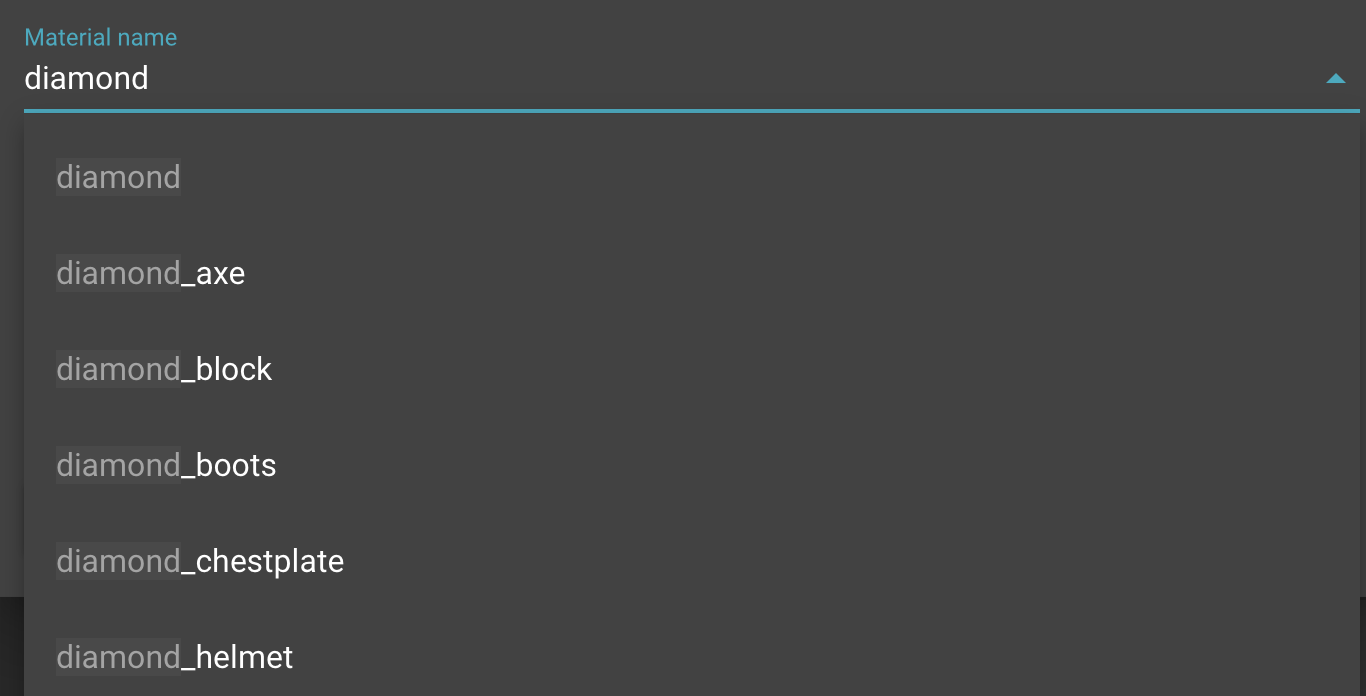
\includegraphics[width=2.5in]{figures/gui_advantage_autocomplete}
\caption{Auto-Completion}
\label{fig:gui_advantage_autocomplete}
\end{figure}

\begin{figure}[!t]
\centering
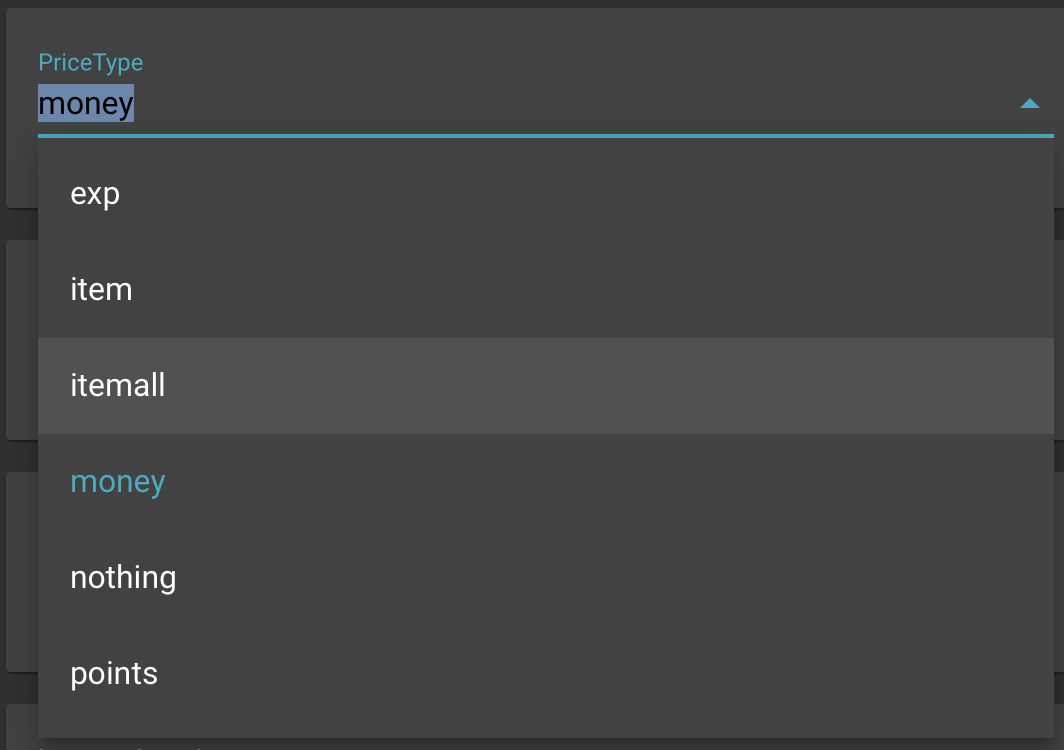
\includegraphics[width=2.5in]{figures/gui_advantage_choiceselection}
\caption{Choice Selection}
\label{fig:gui_advantage_choiceselection}
\end{figure}

%paul
There exist various approaches that generate web forms from a schema, for different frontend frameworks, e.g.,
\textit{React JSON Schema Form}\cite{githubGitHubRjsfteamreactjsonschemaform},
\textit{Angular Schema Form}\cite{githubGitHubJsonschemaformangularschemaform},
\textit{Vue Form Generator}\cite{githubGitHubVuegeneratorsvueformgenerator},
\textit{JSON Forms}\cite{jsonformsMoreForms},
\textit{JSON Editor}\cite{githubGitHubJosdejongjsoneditor}, and
\textit{JSON Form}\cite{githubGitHubJsonformjsonform}.
Those approaches are all based on JSON schema and generate a form that can be filled out by the user and
the resulting JSON document is validated against the schema.
If the user enters invalid data, the form shows an error message.
The generated forms usually have a specific component for each type of data, e.g.\ a text field for strings or a number field for numbers,
similar to our approach.
Figure~\ref{fig:jsonforms} shows an example for a generated form using JSON Forms.

The key differences to our approach are that those editors only provide the GUI for editing the data, but not a text-based editor.
Also, they do not provide an editor for the schema itself.
Finally, all except the last two of the given approaches also require a ``UI schema'' in addition to the JSON schema, which is used to configure the generated form.
While these configurations can be used to customize the generated form, they also add need to be created and maintained by the schema author.
Our approach does only require the JSON schema and does not require any additional configuration, so the user can
use it with any schema file, e.g., from the JSON schema store.

\begin{figure}[htb]
    \centering
    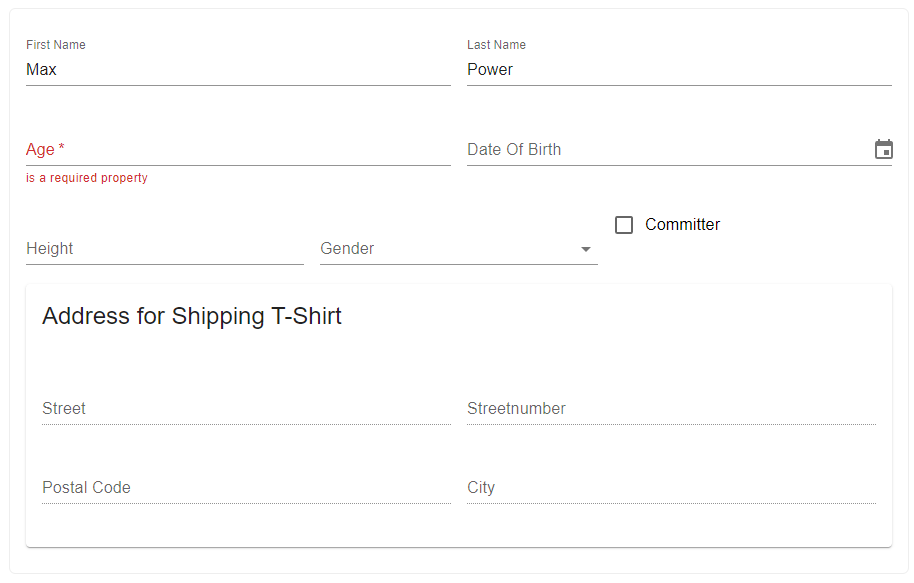
\includegraphics[width=2.5in]{figures/jsonforms}
    \caption{JSON Forms, example for a generated form}
    \label{fig:jsonforms}
\end{figure}

Adamant~\cite{siffa2022adamant} is a JSON-schema based form generator specifically designed for scientific data.
It is similar to our approach in that it generates a GUI from a JSON schema and also allows to edit and create JSON schema documents
and differentiates between a schema edit mode and a data edit mode.
It supports a subset of JSON schema, which is sufficient for many use cases.
In addition to that, it supports the extraction of units from the description of a field, which is useful for scientific data.
Figure~\ref{fig:adamant} shows an example in the schema edit mode.
Adamant differs to \toolname{} in that it does not provide a text-based editor for the schema and that it is specifically designed for scientific data,
while our approach is more general.

\begin{figure}[htb]
    \centering
    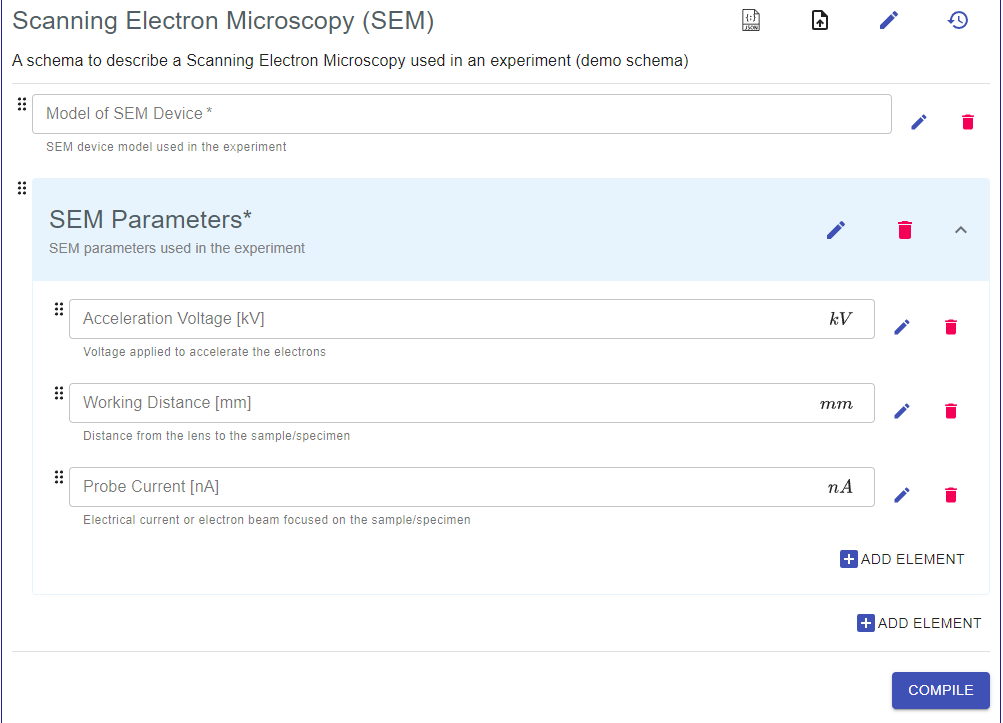
\includegraphics[width=2.5in]{figures/adamant}
    \caption{Adamant, example for a form in edit mode}
    \label{fig:adamant}
\end{figure}


\subsubsection{Schema editors}\label{subsubsec:schema-editors}
In \toolname{} we aim to provide a GUI for both editing \cfgfiles{} and editing the schema.
For the latter, there exist several so-called schema editors, which are tools for creating and editing schemas that are
either text-based or graphical (or both).

The closest to our approach is the \textit{JSON Editor Online}\cite{jsoneditoronlineJSONEditor}, which is a web-based editor for JSON schema.
It divides the editor into two parts, where one part can be used to edit the schema and the other part can be used to edit a JSON document,
which is validated against the schema.
The editor provides various features, such as syntax highlighting and highlighting of validation errors (Figure~\ref{fig:jsoneditoronline}).
It provides a text-based or tree-based view for editing the JSON documents.
For simple objects that are not further nested, it provides also a table-based view (Figure~\ref{fig:jsoneditoronline_table}).
However, the features of the editor are very limited.
For example, it does not provide any assistance for the user, such as tooltips or auto-completion.
For new documents, it does not show the properties of the schema, so the user has to know the schema beforehand.

There also exists variety of schema editors that are paid software, such as \textit{Altova XMLSpy}\cite{altovaEditorXMLSpy},
\textit{Liquid Studio}\cite{liquidtechnologiesJSONSchema}, \textit{XML ValidatorBuddy}\cite{xmlbuddyEditorValidator},
\textit{JSONBuddy}\cite{jsonbuddyJSONSchema}, \textit{XMLBlueprint}\cite{xmlblueprintEditorXMLBlueprint},
and \textit{Oxygen XML Editor}\cite{oxygenxmlCompleteSolution}.
Those are editors for XML or JSON schema, mostly with a combination of text-based and graphical views.
In contrast to our approach, they are not web-based and do not focus on editing a JSON document based on a schema,
but rather on editing the schema itself.
In this regard, they are more specialized than our approach.

\subsubsection{Schema visualization}\label{subsubsec:schema-visualization}
Generating a GUI from a schema is related to schema visualization, for which several techniques exist~\cite{Frasincar2006, SILVA201928, 10.1145/1317353.1317362, 1173142}.
However, with schema visualization the focus is only on providing a static visual representation of the schema
and not on providing a GUI for editing the schema.
Thus, we do not consider schema visualization approaches in this work.
However, future work could investigate how such techniques could be embedded in our approach.

\begin{figure}[htb]
    \centering
    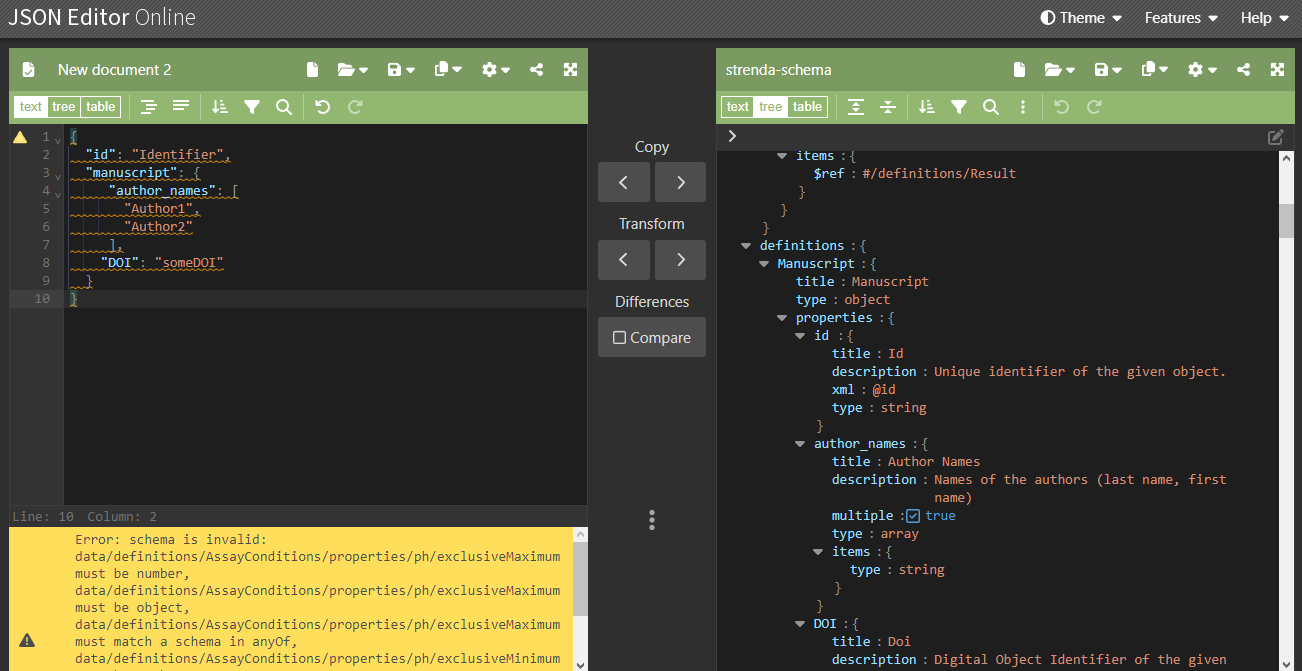
\includegraphics[width=2.5in]{figures/jsoneditoronline}
    \caption{JSON Editor Online}
    \label{fig:jsoneditoronline}
\end{figure}
\begin{figure}[htb]
    \centering
    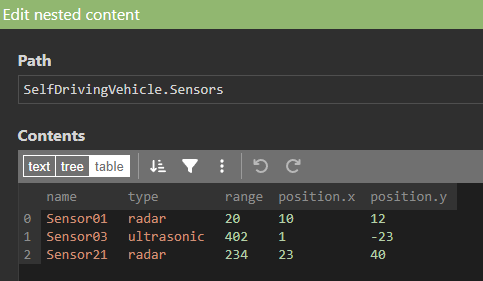
\includegraphics[width=2.5in]{figures/jsoneditoronline-table}
    \caption{JSON Editor Online}
    \label{fig:jsoneditoronline_table}
\end{figure}

% Minye
% todo more details
% adamant is specific for science context -> would be interesting
% it also extracts the unit from the description -> also interesting
% also how are they different from our approach?
%\begin{enumerate}[label=(\alph*)]
%    \item \textbf{Vue Form Generator}\cite{vueformgenerator}: is a schema-based form generator component for Vue.js.
%    It can be extended with custom fields.
%    At the time of writing this paper the tool was rated with most stars among web form generator projects. % todo reword maybe
%
%    \item \textbf{JSON Forms}~\cite{JSONForms}: is a declarative framework for building form-based web UIs.
%    It can be integrated with UI libraries or frameworks, such as Vue, React or Angular.
%
%    \item \textbf{Adamant}~\cite{siffa2022adamant}: also is a JSON-schema based form generator, that supports any valid schema.
%    It also supports schema validation.
%
%\end{enumerate}

% paul



\section{Evaluation of Schema Languages}\label{sec:evaluation-of-schema-languages}


We evaluate the schema languages mentioned in section~\ref{subsec:schemalanguages} to determine which is the most suitable one for this work.


\subsection{Evaluation criteria}\label{subsec:evaluation-criteria} % evaluation by paul, some criteria ideas by felix

Ideally, the schema language of \toolname is both popular and supported by numerous tools and libraries as well as expressive enough to express the features we need.
We use the following criteria and metrics:
\begin{enumerate}
% metric: Stackoverflow question # with schema language as tag
    \item \textbf{Practical usage} --- Ideally our approach uses a schema language that already known by many developers.
    As indicator of the practical usage we use the approximate search results on stackoverflow.com as metric.
    We acquire the results by querying the google search engine with the name of the schema language and ``site:stackoverflow.com'', which limits the search results to stackoverflow.com.
    This metric might also correlate with the complexity of the schema language as a more complex to use schema language will likely lead to more questions asked on the site.
    Nevertheless, we assume that a significantly higher number of results indicates that a language is more known than others.

    Additionally, we investigate how well the schema languages are supported by IDEs and code libraries:
    \begin{enumerate}
        \item \textit{Tool support} --- We used the 10 most popular IDEs\cite{mostpopularides} and checked if the IDE supports the schema language either natively or by a plugin.
        Support here means that either the IDE is capable of validating documents against a schema in the schema language or supports creating schema files, e.g., by using syntax highlighting for the schema language.
        % # node modules with schema language keyword....
        \item \textit{Library support} --- As we implement a web-based tool, we JavaScript or TypeScript bases tools are helpful for our approach, e.g., so we can reuse a package for schema validation.
        We investigate the number of node modules exist that are related to the schema languages by querying the node module search on \url{www.npmjs.com} with the name of the schema language.

    \end{enumerate}

    % # of cases fulfilled from below
    \item \textbf{Expressiveness} --- We evaluate how expressive each of the schema languages are, i.e., what possible constructs the language is able to express.
    We define eight requirements on the language features that we consider helpful for our approach.
    The number of requirements a schema language fulfills is our metric that indicates how expressive the language is.
    Table~\ref{tab:comparison} reports the results.
    The nine requirements are:
    \begin{enumerate}
        \item \textit{Simple types} --- This is fulfilled if the schema language provides the possibility to define simple data types, at least strings, numeric types, and a boolean type.
        This is a fundamental feature for our approach.
        \item \textit{Complex types} --- This is fulfilled if the schema language provides the possibility to define complex data types, at least records and arrays.
        This is crucial feature for our approach as configuration files are often structured data rather than plain key-value pairs.
        \item \textit{Descriptions} --- This is fulfilled if the schema language provides the possibility to add descriptions to fields.
        This is helpful in a schema-to-GUI approach as the description can be shown to the user, providing potential helpful information on how a field should be filled.
        \item \textit{Examples} --- This is fulfilled if the schema language provides the possibility to add example values.
        This is helpful in our approach as the example values can serve as placeholders in the GUI editor.
        \item \textit{Default values} --- This is fulfilled if the schema language provides the possibility to add default values which are assumed in an absence of a value.
        This often helpful information can be displayed to the user or used as placeholder values.
        \item \textit{Optional values} --- This is fulfilled if the schema language provides the possibility to declare values as optional or required.
        Often it is not necessary to provide all values in a configuration file, so it is helpful to mark fields as required or optional in the GUI editor.
        \item \textit{Constraints} --- This is fulfilled if the schema language provides the possibility to constrain values of fields, e.g., maximum length of strings.
        To be exact, for this evaluation we required that at least two of the following constrained can be expressed by the schema language:
        \begin{itemize}
            \item The length of strings can be limited.
            \item The range of numeric types can be limited, e.g., to only positive values.
            \item The valid values of a field can be restricted to a finite amount of values (enumeration).
            \item The format of a string field can be constrained to a certain pattern.
        \end{itemize}
        This is a helpful feature for our approach as often not all possible values are valid for specific fields in configuration files.
        \item \textit{Conditions} --- This is fulfilled if the schema language provides the possibility to define conditional dependencies between fields.
        This is a advanced feature that is helpful because it allows to express for example that a particular field must be given only if another field has a specific value.
        \item \textit{References} --- This is fulfilled if the schema language provides the possibility to define reusable subschemas that can be referenced in other parts of the schema.
        This is often useful in practice to reuse common data structures.

    \end{enumerate}

    %\item \textbf{Support for XML, YAML, or JSON} ---

    % For our approach we aim to use the same or at least a very similar editor for both editing the actual \cfgfiles and the schema files. Consequently, the schema language should be a subset of the language that the \cfgfiles are written in, i.e. the document language. For example JSON schema files are JSON files and JSON schema is used to validate JSON files, so here this criteria is fulfilled. In constrast, DTD is a schema language for validating XML files but a DTD file is not a valid XML file.

\end{enumerate}


    \begin{table*}[]
    \centering
    \caption{Evaluation of different schema languages\label{tab:all}}
        \begin{tabular}{@{}lrrrr@{}}
        \toprule
        \textbf{Schema language} &
          \textbf{\# Search results } &
          \textbf{IDE support} &
          \textbf{\# Node packages} &
          \textbf{Expressiveness} \\ \midrule
        JSON schema &
          245.000 &
          8 / 10 &
          4.536 & 9 /9 \\
        XSD & 151.000 & 8 / 10 & 116 & 8 / 9 \\
        DTD & 69.700 & 9 / 10 & 34 & 6 / 9 \\
        CUE & 10.500 & 4 / 10 & 97 &   8 / 9 \\
        Avro & 20.000 & 8 / 10 & 211 &  5 / 9 \\
        JSON Type Definition (JTD) &  109 & 0 / 10 &  17 & 5 / 9 \\
        TypeSchema &  8.450 & 0 / 10 & 5 & 8 / 9 \\
        protobuf &  44.800 & 9 / 10 & 1.210 & 4 / 9 \\
        GraphQl schema & 31.000 & 7 / 10 & 1.509 & 6 / 9\\ \bottomrule
        \end{tabular}
    \end{table*}
    %\label{fig:my_label}
%\end{figure}

% IDE                | JSON schema | XSD | DTD | CUE | Avro | protobuf | GraphQL schema |
% Visual Studio      | yes         | yes | yes | x   | yes  | yes      | yes            |
% Visual Studio Code | yes         | yes | yes | yes | yes  | yes      | yes            |
% Eclipse            | yes         | yes | yes | x   | yes  | yes      | x              |
% pyCharm            | yes         | yes | yes | yes | yes  | yes      | yes            |
% Android Studio     | yes         | yes | yes | yes | yes  | yes      | yes            |
% IntelliJ           | yes         | yes | yes | yes | yes  | yes      | yes            |
% NetBeans           | x           | yes | yes | x   | x    | yes      | x              |
% RStudio            | x           | x   | x   | x   | x    | x        | x              |
% Atom               | yes         | x   | yes | x   | yes  | yes      | yes            |
% Sumblime Text      | yes         | yes | yes | x   | yes  | yes      | yes            |
% ======================================================================================|
%                    | 8 / 10      | 8   | 9   | 4   | 8    | 9        | 7              |

\begin{table*}
    \centering
    \caption{Comparison of expressiveness of different schema languages
    \label{tab:comparison}}
    \begin{tabular}{@{}llllllllllr@{}}
        \toprule
        \textbf{Schema language} &
          \thead{Simple \\ types} &
          \thead{Complex \\ types} &
          \thead{Descriptions} &
          \thead{Example \\ values} &
          \thead{Default \\ values} &
          \thead{Optional \\ values} &
          \thead{Constraints} &
          \thead{Conditions}  &
          \thead{References}  &
          \thead{Result}\\ \midrule
        JSON schema &
          \checkmark &
          \checkmark &
          \checkmark &
          \checkmark &
          \checkmark &
          \checkmark &
          \checkmark &
          \checkmark &
          \checkmark & 9 / 9\\
        XSD &
          \checkmark &
          \checkmark &
          \checkmark &
          x &
          \checkmark &
          \checkmark &
          \checkmark &
          \checkmark &
          \checkmark & 8 / 9 \\
        DTD &
         \checkmark &
         \checkmark &
         x &
         x &
         \checkmark &
         \checkmark &
         x &
         \checkmark &
         \checkmark & 6 / 9\\
        CUE &
         \checkmark &
         \checkmark &
         \checkmark &
         \checkmark &
         x &
         \checkmark &
         \checkmark &
         \checkmark &
         \checkmark & 8 / 9\\
        Avro &
         \checkmark &
         \checkmark &
         x &
         x &
         \checkmark &
         \checkmark &
         x &
         x &
         \checkmark & 5 / 9\\
        JTD &
         \checkmark &
         \checkmark &
         x &
         x &
         x &
         \checkmark &
         x &
         \checkmark &
         \checkmark & 5 / 9\\
        TypeSchema &
         \checkmark &
         \checkmark &
         \checkmark &
         x &
         \checkmark &
         \checkmark &
         \checkmark &
         \checkmark &
         \checkmark & 8 / 9\\
        protobuf &
            \checkmark &
            \checkmark &
            x &
            x &
            x &
            \checkmark &
            x &
            x &
            \checkmark & 4 / 9 \\
        GraphQL schema &
         \checkmark &
         \checkmark &
         \checkmark &
         x &
         \checkmark &
         \checkmark &
         x &
         x &
        \checkmark & 6 / 9\\
          \bottomrule
    \end{tabular}
\end{table*}

% paul
\subsection{Evaluation results}\label{subsec:evaluation-results}

Tables~\ref{tab:all} and \ref{tab:comparison} show the results of our evaluation.
We come to the conclusion that JSON schema is sufficiently popular and expressive that we choose to use it as the schema language for our approach.
The other schema languages are either less expressive or less popular.
This result is in line with the work of Baazizi et al.~\cite{baazizi2021empirical}, who also found over 80.000 JSON schema files on GitHub,
and with the claim of the JSON schema website\cite{jsonschemaJSONSchema} that JSON schema is the de-facto standard for JSON schema languages.

% paul

%\subsection{Schema inference}\label{subsec:schema-inference}
%
%Schema inference is the process of deriving a schema from existing data.
%For our use case, this means inferring JSON schema from JSON documents.
%Frozza et al.~\cite{8424731} and Klettke et al.~\cite{klettke} present algorithms for JSON schema inference from JSON data of NoSQL data storages.
%Baazizi et al.\cite{Baazizi2019} also investigate schema inference from massive data sets but their approach uses its own type system rather than JSON schema.
%
%In our tool we only aim to infer a schema from a single sample, as an optional assisting feature for our users, for which various libraries exist~\cite{githubGitHubJsonsystemspublic, githubGitHubSaasquatchjsonschemainferrer, probst_siegel_2023}.



 \section{Design}\label{sec:design}
 % TODO (but maybe not here?): explain why and how we define our own meta schema based on json schema, because we use just subset of its features and because our schema is used to generate schema editor GUI and therefore should only show what is supported. Also we want to add descriptions and maybe more. Also limit options to not overwhelm and confuse the user.
% TODO also describe more the users perspective how users would use the tool?

% felix
\subsection{User Interface}\label{subsec:overview}
The design of \toolname{} is inspired by another tool\cite{githubBspEditor} by one of the authors, which is a GUI program that assists users in editing configuration files for the Minecraft server plugin BossShopPro\cite{bossshoppro}.
That tool provides the user a code panel for editing configuration files of that domain in a text editor, as well as a GUI panel, where the user can edit their configuration file using GUI components.
\toolname{} differs from that tool by being generic, instead of being bound to a certain domain, by having a much more expressive schema language, a schema editor and many other features that improve the user experience, such as a search functionality.
%TODO: maybe move to related work?

Before we dive into the architecture and detailed design of \toolname{}, this section provides an overview from the view of the user.

The user interface has three distinct views:
\begin{enumerate}
	\item File editor (figure \ref{fig:fileeditor}): In this view the user can modify their \cfgfile{}, based on a schema.
	\item Schema editor (figure \ref{fig:schemaeditor}): In this view the user can modify their schema.
	\item Settings (figure \ref{fig:settings} in appendix): In this view the user can adjust parameters of the tool.
\end{enumerate}


\begin{figure*}
    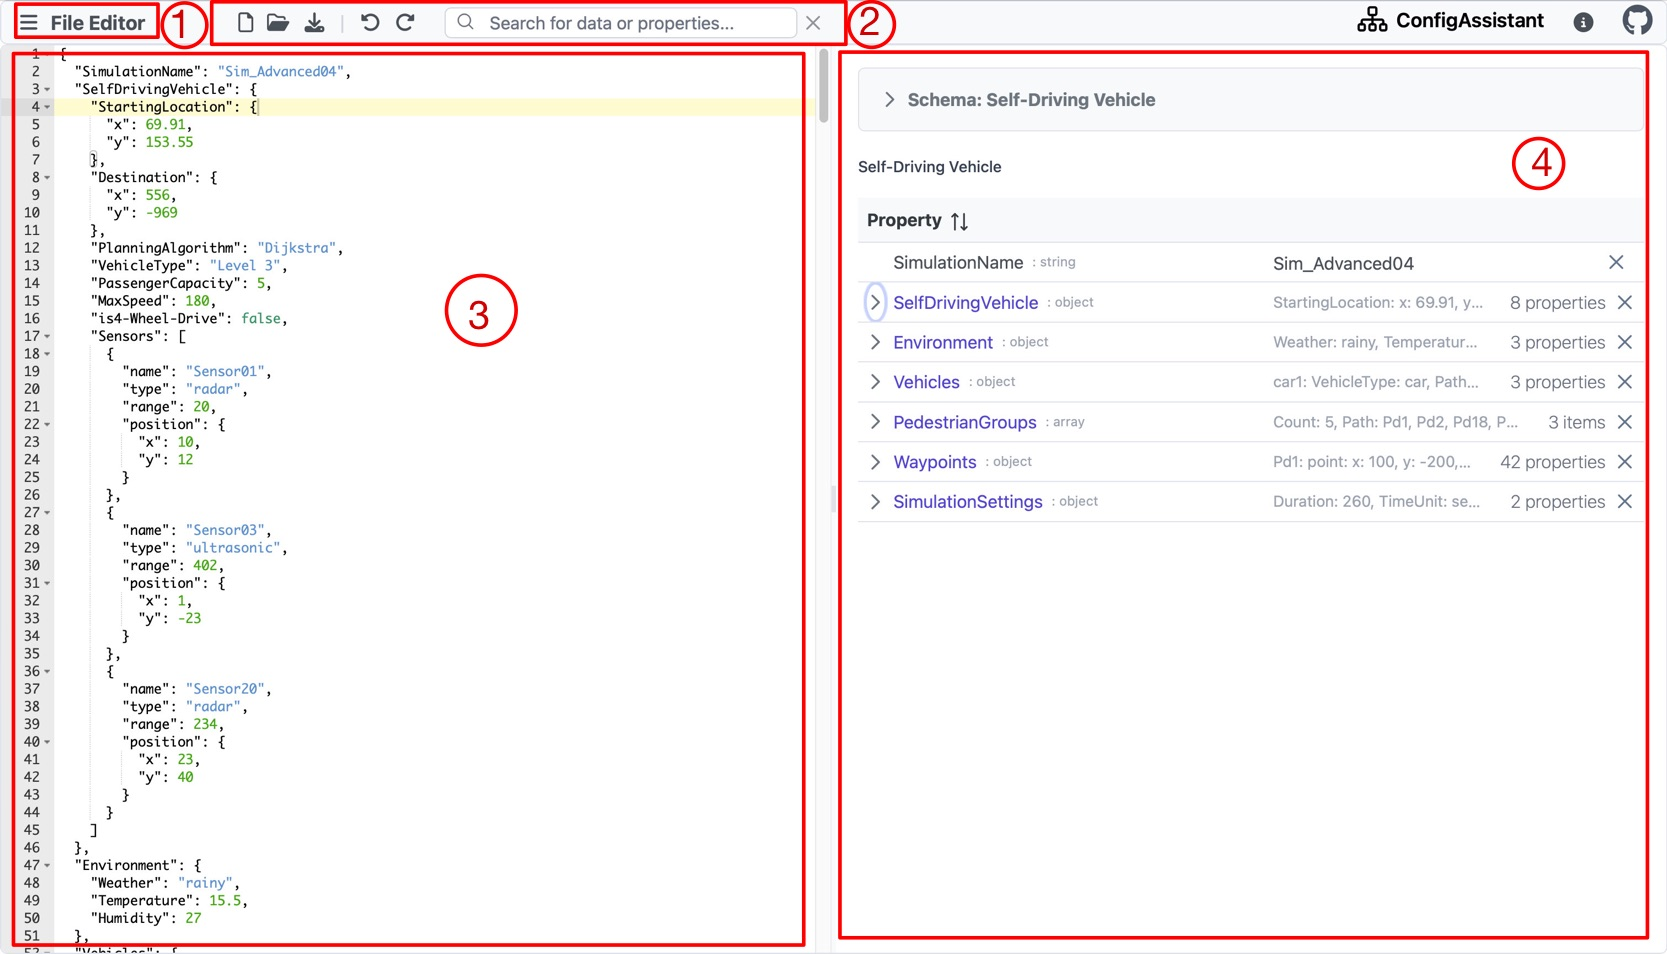
\includegraphics[width=\textwidth]{figures/fileeditor}
    \caption{UI of file editor view. Different components highlighted in red: 1) button to switch to other view (e.g. to Schema Editor view), 2) Toolbar with various functionality, 3) Code panel, 4) GUI panel}
    \label{fig:fileeditor}
\end{figure*}

\begin{figure*}
    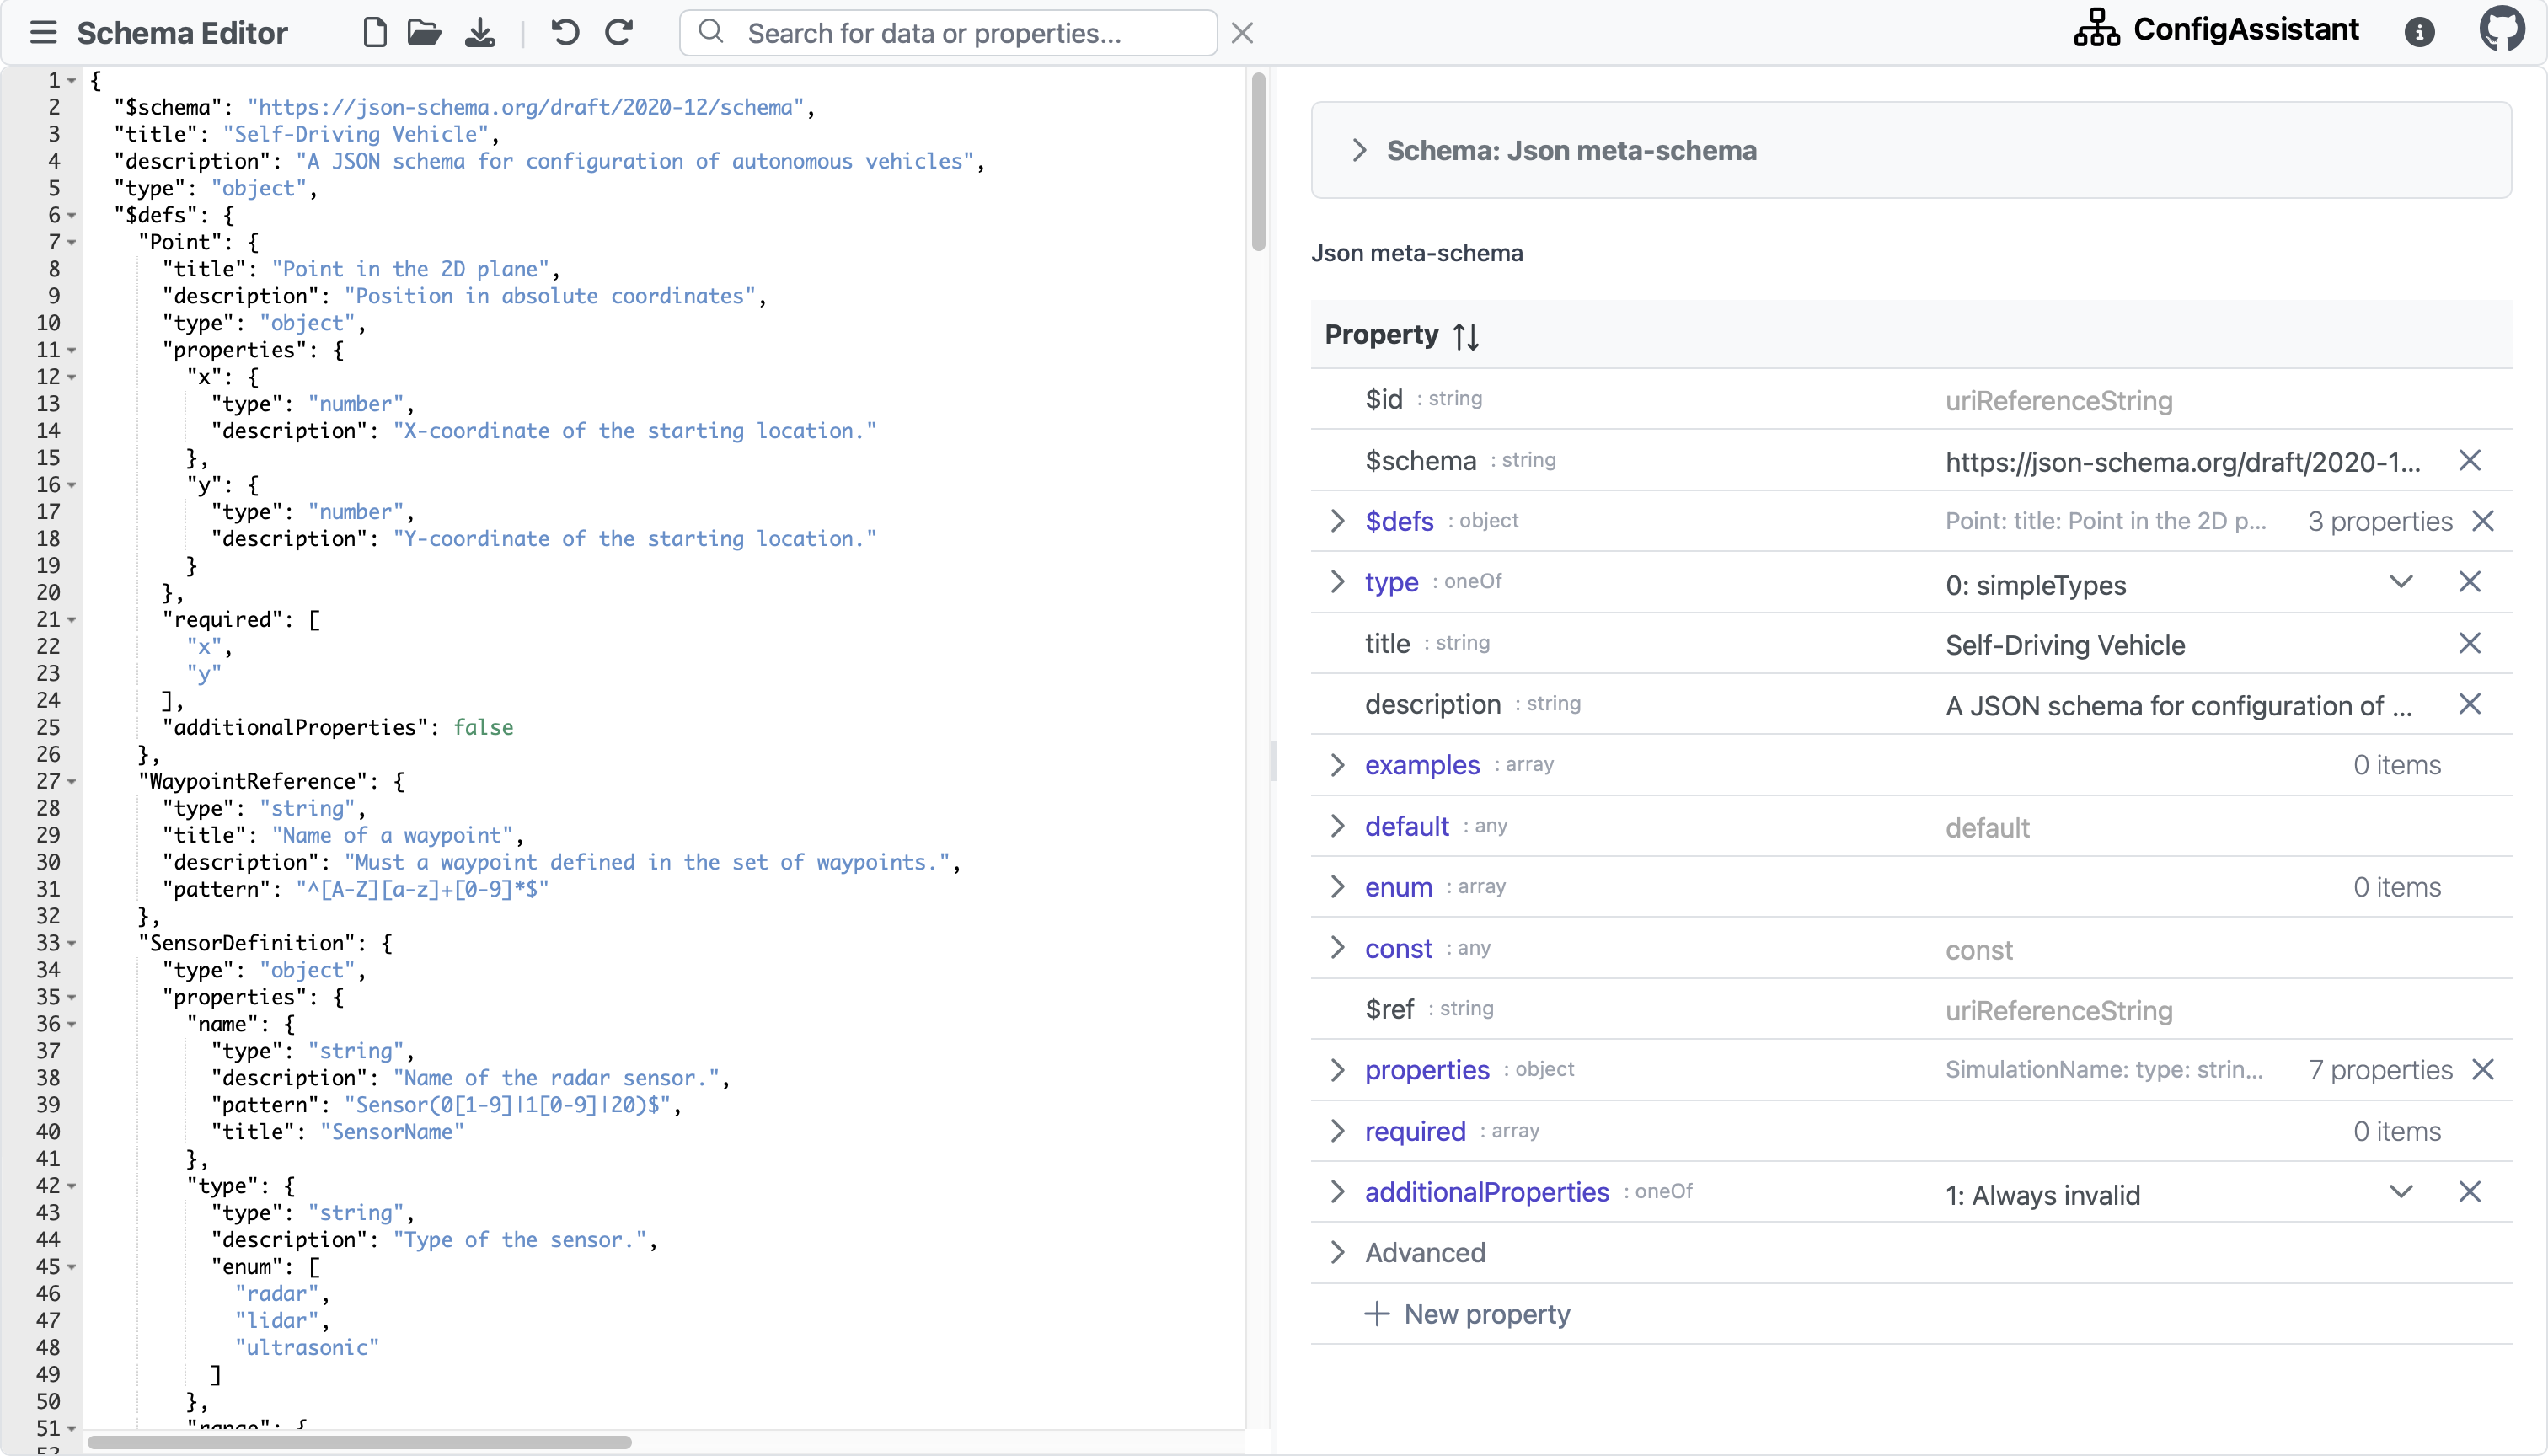
\includegraphics[width=\textwidth]{figures/schemaeditor}
    \caption{UI of schema editor view}
    \label{fig:schemaeditor}
\end{figure*}


The UI is divided into two main panels: the  \textit{Code panel} (on the left) and the \textit{GUI panel} (on the right).
In the \textit{Code panel} the user can modify their data by hand, as in a regular code editor.
Features, such as syntax highlighting and schema validation, assist the user.
In the \textit{GUI panel}, the user can modify their data with the help of a GUI.
The GUI is based on the schema which the user provides (more on that in the next paragraphs).
For example, for enum properties, the user will get a dropdown menu with the different options to choose from and for boolean properties the user will get a checkbox.
Other features, such as tooltips that display the description and constraints of a property, further assist the user.

This design combines the benefits of both a rich text code editor (efficient for many tasks, more suited for users with technical understanding of the data structure) with the benefits of a GUI (enables users without deep technical understanding to work with the data, assists also expert users).

As a schema is a \cfgfile{} itself, it can be treated as such and the tool can offer assistance accordingly.
Note that whenever the user edits a \cfgfile{} using the tool, they do so using some underlying schema.
Even the tool settings can be seen as a \cfgfile{}, for which the underlying schema is a settings schema.

Table \ref{tab:schema_and_file_data_by_mode} illustrates how for the different views, file data and schema being used by the tool differ.
\begin{table}[!t]
\caption{File data and schema for the different views}
\label{tab:schema_and_file_data_by_mode}
\centering
\begin{tabular}{lll}
\toprule
\textbf{View} & \textbf{Effective File Data} & \textbf{Effective Schema} \\
\midrule
File editor   & User data                    & User schema               \\
Schema editor & User schema                  & JSON Meta Schema          \\
Settings      & Settings data                & Settings schema           \\
\bottomrule
\end{tabular}
\end{table}


\subsection{Intended Workflow}\label{subsec:workflow} %keyuri
\begin{enumerate}
    \item Upon initial access of \toolname{}, a dialog is displayed, where users can select their desired schema.
    \item After selecting a schema, the user will find that a GUI is automatically generated on the right-hand side of the file editor,
    tailored to the selected schema.
    \item Through the GUI panel, users are assisted in creating or modifying \cfgfiles{}.
    \item If a user wishes to modify the selected schema, such as adding new properties, they can do so through the schema editor.
    Changes can be made using either the GUI panel or the code panel, and these modifications will automatically reflect in the file editor.
\end{enumerate}

%\begin{figure}[!htb]
%    \begin{minipage}[t]{0.5\textwidth}
%        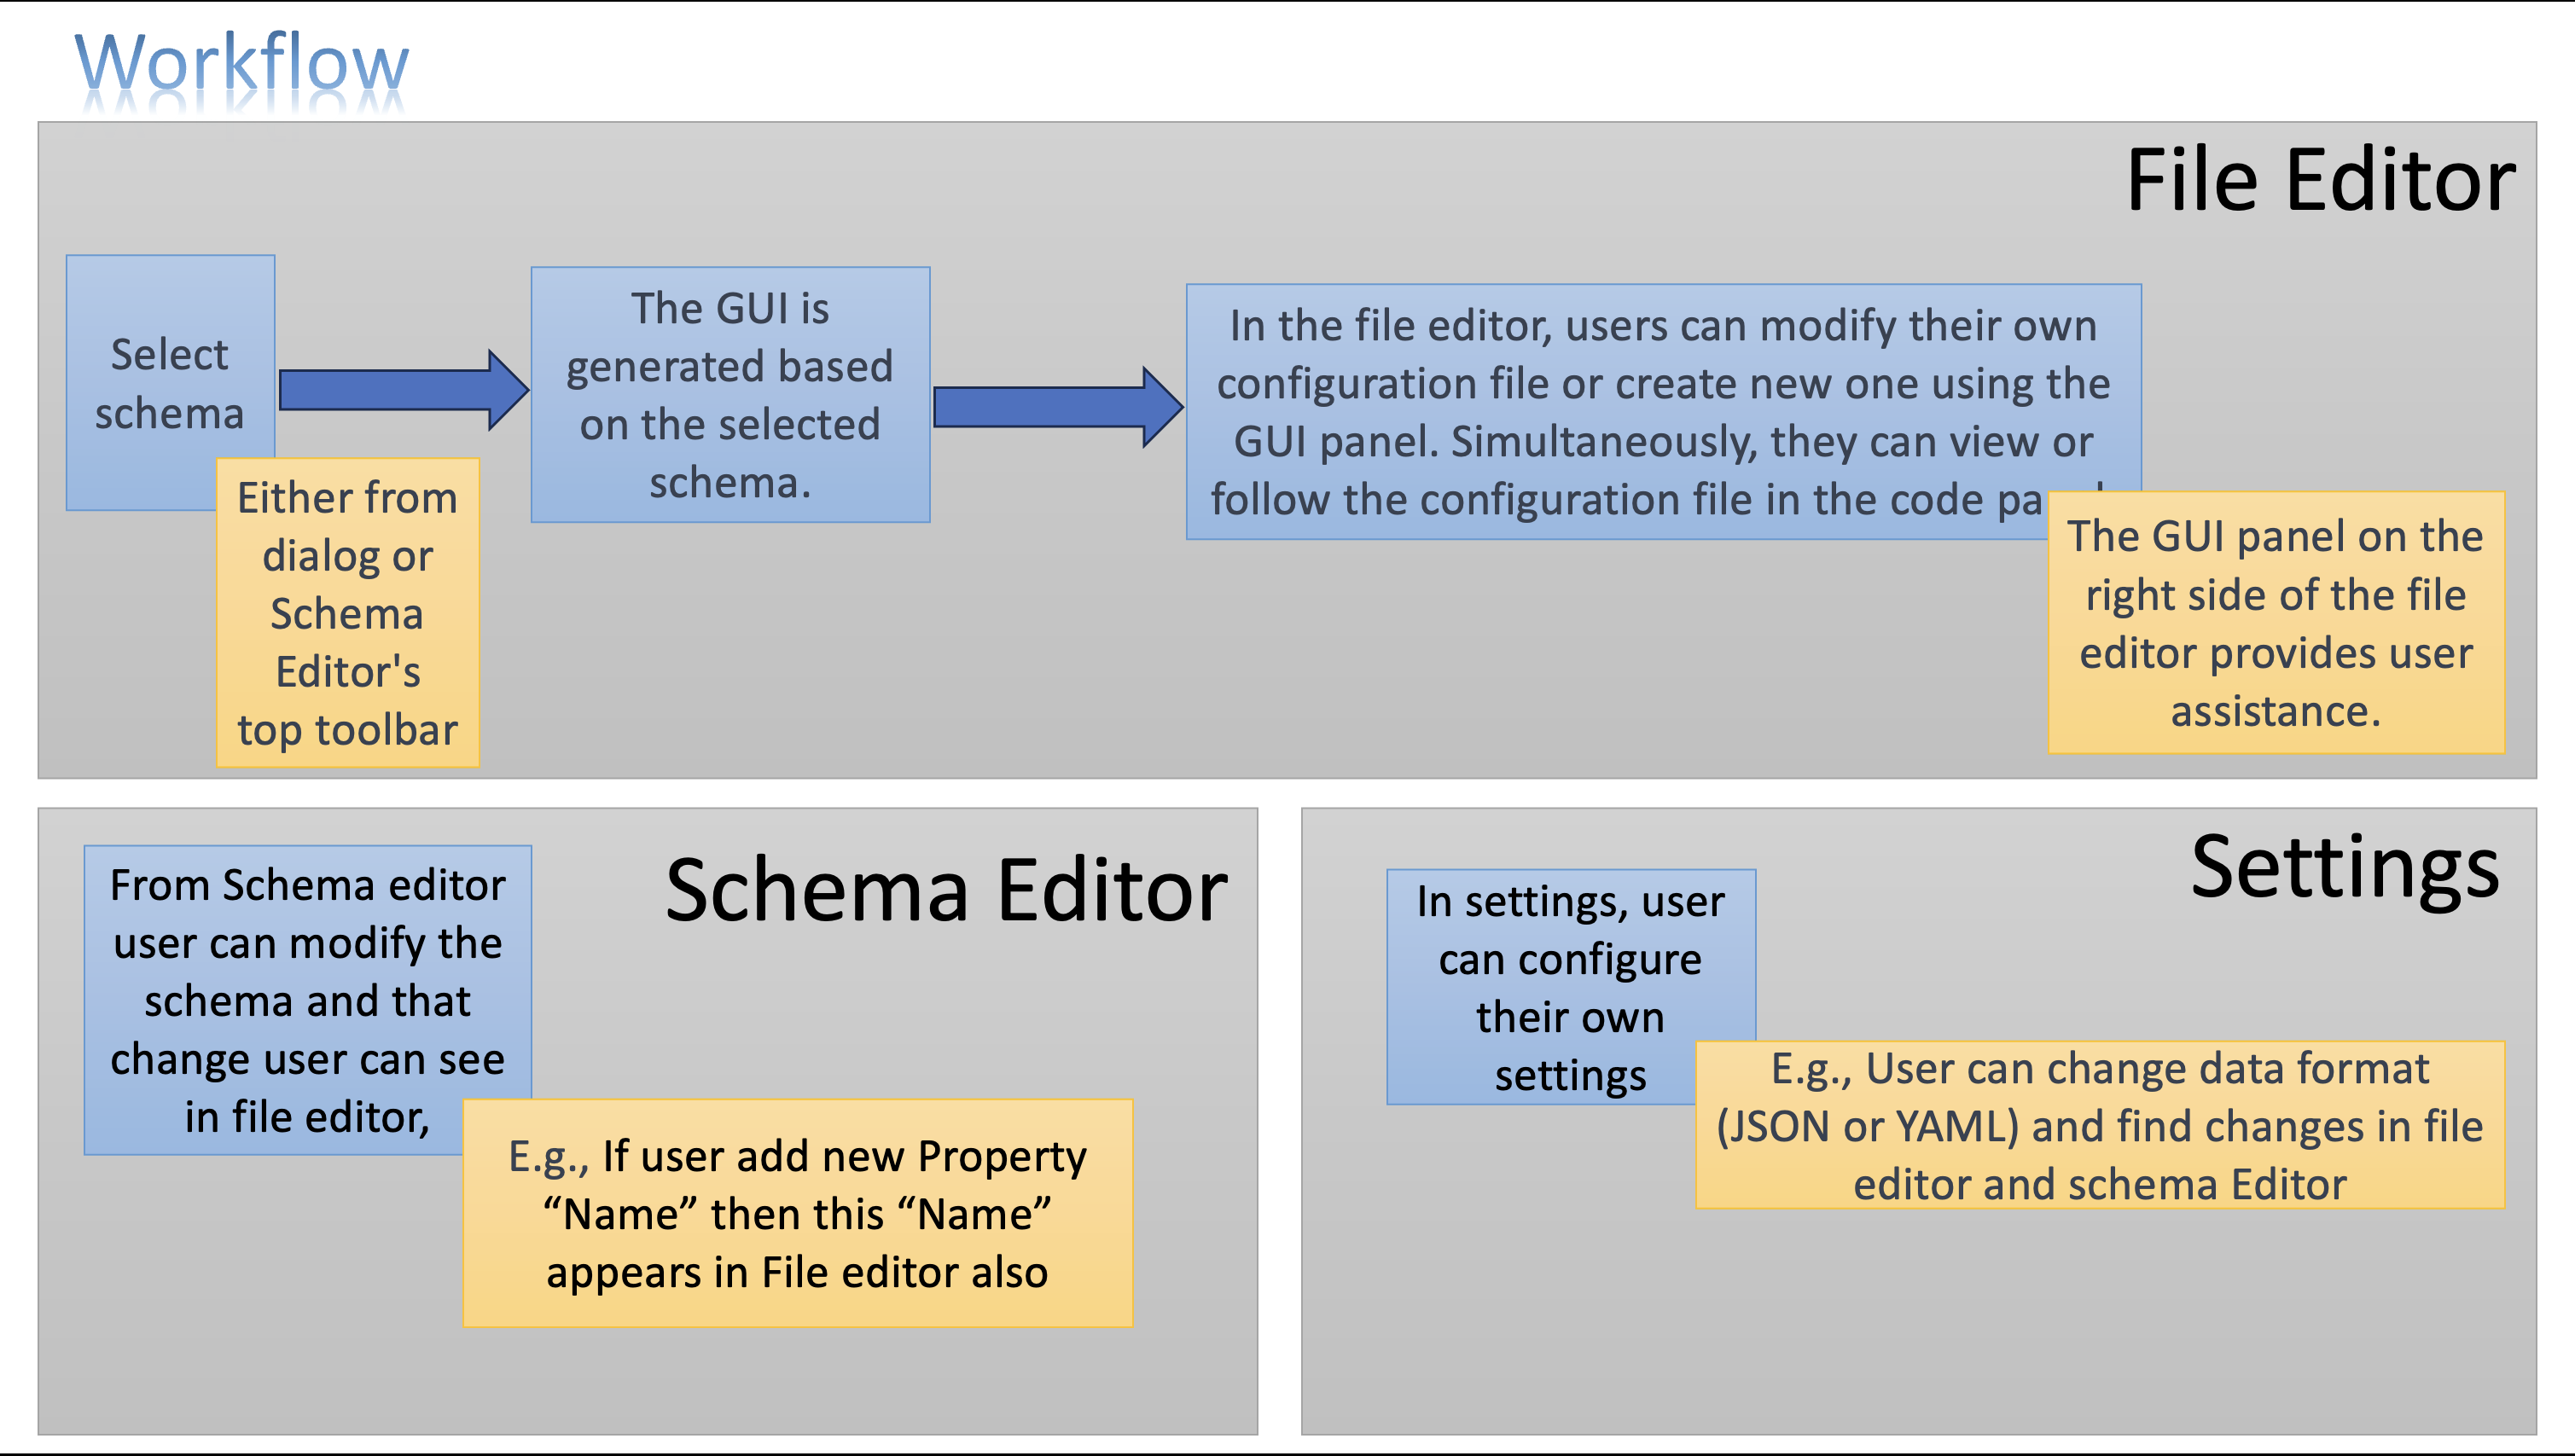
\includegraphics[width=3.5in]{figures/Toolworkflow}
%        \caption{Workflow}
%        \label{workflow}
%    \end{minipage}\label{fig:workflow}
%\end{figure}




% felix

\subsection{Architecture}\label{subsec:architecture} % todo diagram illustrating the architecture
This section describes our main architectural design decisions.
Those will not be relevant or visible for the user of the tool, but are important for understanding our implementation.
Aim of those design decisions is to ensure modularity and maintainability of the tool.

The core of \toolname{} is a single source of truth data store that contains the current user configuration data (as a JavaScript Object).
With this data store we can bidirectionally connect what we call ``editor panels''.
An editor panel is a modular component that the user of the tool can access to modify the config data in an indirect way.
It might be implemented as a code editor, a graphical user interface or any other way in which the data can be presented to the user.
All editor panels are independent and do only have access to the data store but not to each other.
Every editor panel subscribes to the changes of the data store, so it can be updated accordingly whenever the data in the store is changed.
Additionally, every panel has the capabilities of updating the data store themselves, which is done when the user modifies the data in the editor panel.
The following artificial example use-cases illustrate the capabilities of this architecture:

\begin{itemize}
    \item Format converter: one panel shows the data in a code editor in JSON format, a second panel shows the data in a code editor in YAML format. Any semantic data change on one panel will cause the same semantic change in the other panel.
    \item Split-Screen Editor: one panel shows the data in a code editor, a second panel shows the data in a GUI. This way the user can have the efficiency of a text editor, but also the assistance of a GUI at the same time. Any semantic data change on one panel will be forwarded to the other panel.
    \item The Split-Screen Editor could be implemented for different data formats, such as YAML, JSON and XML. The architecture allows any data format as long as there exists a mapping from this data format to a JavaScript Object and back.
\end{itemize}

In practice, we implement only one code editor panel, as well as one GUI editor panel.
The architecture, however, would be flexible enough to allow replacing any of these panels or adding new ones, since they are decoupled from each other and only communicate with the single source of truth data store.

% TODO: Add diagram with store in center in several panels with bidirectional connection of subscribe/update

% felix

\subsubsection{Single Source of Truth Data Store}
This is the core of the tool.
The panels can subscribe to this store to receive updates whenever data is changed.
Also, panels can trigger changes of the data in the store.
Besides the current configuration data, the store also stores the path of the currently selected data entry and the schema that is currently being used.

% felix

\subsubsection{Code Panel}\label{subsubsec:design_text_editor_panel}
For the code panel, we embed a rich-text code editor that already supports syntax highlighting and other useful features.
We enable validation of whether the text is well-formed according to the JSON/YAML/XML standard and add schema validation.
The panel subscribes to the data store.
Whenever the configuration data is changed in the store, the panel will take the new configuration data JavaScript Object, serialize it into the given data format and replace the text in the code editor with the new serialized data.
The action of replacing the text in the code editor will cause formatting and comments to be lost, which we accept.
In the future, several mechanisms can be applied to avoid the loss of formatting or comments (see section \ref{subsec:future-work}).

When the user edits the text in the code editor, the text is deserialized into a JavaScript Object and sent to the data store, which then updates the configuration data object and notifies all other subscribed panels of the change.


To enable communication with the store, for any data format that the tool should support, we need a function to stringify a JavaScript object to a string in the data format and a function to parse a string in that data format as a JavaScript object.


To make it possible to highlight certain lines in the editor as erroneous (schema violations) or jump to certain lines (e.g. when the user selects a property in the GUI editor, we want to jump to the same property in the text editor), we need a function \texttt{determineRow(editorContent, dataPath)} that can determine the corresponding editor line, based on the configuration text and a given data path.

The other way around, when the user places their cursor inside the text editor, we want to determine the path of the element that the cursor is currently at. This requires a function \texttt{determinePath(editorContent, cursorPosition)} which returns a data path based on the configuration text and a given cursor position.

% felix

\subsubsection{GUI Assistance Panel}
The GUI assistance panel directly works with the given schema and provides the user with corresponding GUI elements, such as a checkbox for a boolean data structure or a text field for a string data structure.
Additional GUI elements, such as tooltips (showing the description of a data field) are used to support the easier.
The GUI elements are constructed in the following manner: a schema is seen as a hierarchical tree of data field definitions and their corresponding constraints.
A data field can either be simple (string, boolean, number, integer) or complex (array or object with children).
Every schema has a root data field.
The GUI element for this root data field is constructed.
When constructing the GUI element for a complex data field, all GUI elements of the child data fields are constructed too, in a recursive manner.
This way, the whole schema tree is traversed and GUI elements for all entries are constructed.
To avoid overwhelming the user with too many GUI elements, the ones with child elements can be expanded or collapsed by the user and only a limited amount of them is expanded by default.
By design, each of these constructed GUI elements is mapped to their corresponding data field (in other words: to a path in the data structure).
The initial values of all GUI elements are taken from the data in the store, by accessing the data at the given paths.
Whenever the values in a GUI element are adjusted by the user, the data in the store will be updated with the new values.





 \section{Implementation}\label{sec:implementation}
 We use vue.js (TODO citation) as the UI framework for our tool, combined with PrimeVue (TODO citation) as the UI component library and Tailwind CSS (TODO citation) for CSS utility.
A detailed list of all libraries used can be found in the wiki of our GitHub repository (TODO link).
Table~\ref{tab:libraries} shows an overview of the most important libraries used and their purpose.

% todo insert most important libraries used and their purpose
\begin{table*}[!hb] % Use table* for wide tables
    \caption{Libraries used in the implementation of our tool} %keyuri
    \label{tab:libraries}
    \centering
    \begin{tabular}{ll}
        \toprule
        \textbf{Library} & \textbf{Purpose}     \\
        \midrule
        vue.js           & UI framework         \\
        PrimeVue         & UI component library \\
        Tailwind CSS     & CSS utility          \\
        @fortawesome/fontawesome-svg-core & Font Awesome SVG icons. \\
        ajv@8.12.0 & JSON schema validator for Node.js and browsers. \\
        brace@0.11.1 & Browser-based code editor with syntax highlighting and code folding. \\
        primeicons@6.0.1 & It is a popular UI component library for JavaServer Faces (JSF) applications. \\
        \bottomrule
    \end{tabular}
\end{table*}

\subsection{Tool Overview}\label{subsec:tool-overview} %keyuri


The tool provides a solution for managing \cfgfiles{} with three distinct views:
\begin{itemize}
    \item \textbf{File Editor} (Figure~\ref{fig:fileeditor}): For editing \cfgfiles{}, based on the schema provided to the tool.
    \item \textbf{Schema Editor} (Figure~\ref{fig:schemaeditor}): For editing the schema, which is used by the File Editor.
    \item \textbf{Settings} (Figure~\ref{fig:settings}): To configure various tool settings.
\end{itemize}

The user interface of \toolname{} is structured in the following way (see the numbers in red in figure~\ref{fig:fileeditor}):
\begin{enumerate}
    \item Button to switch to another view (e.g., from File Editor to Schema Editor).
    \item Toolbar with various functionality.
    \item Code editor panel.
    \item GUI editor panel.
\end{enumerate}
% While these views may share a similar appearance in the figure, each number assigned to them serves a distinct purpose.
% The first number corresponds to different views, allowing users to switch between the Schema Editor,File Editor and Settings, the second number pertains to the toolbar, functionalities for each view listed following, the third number represents the Code Panel, and the fourth number designates the GUI Panel on the right. We will discuss the unique functions of each of these views in the following sections.

\begin{figure*}
    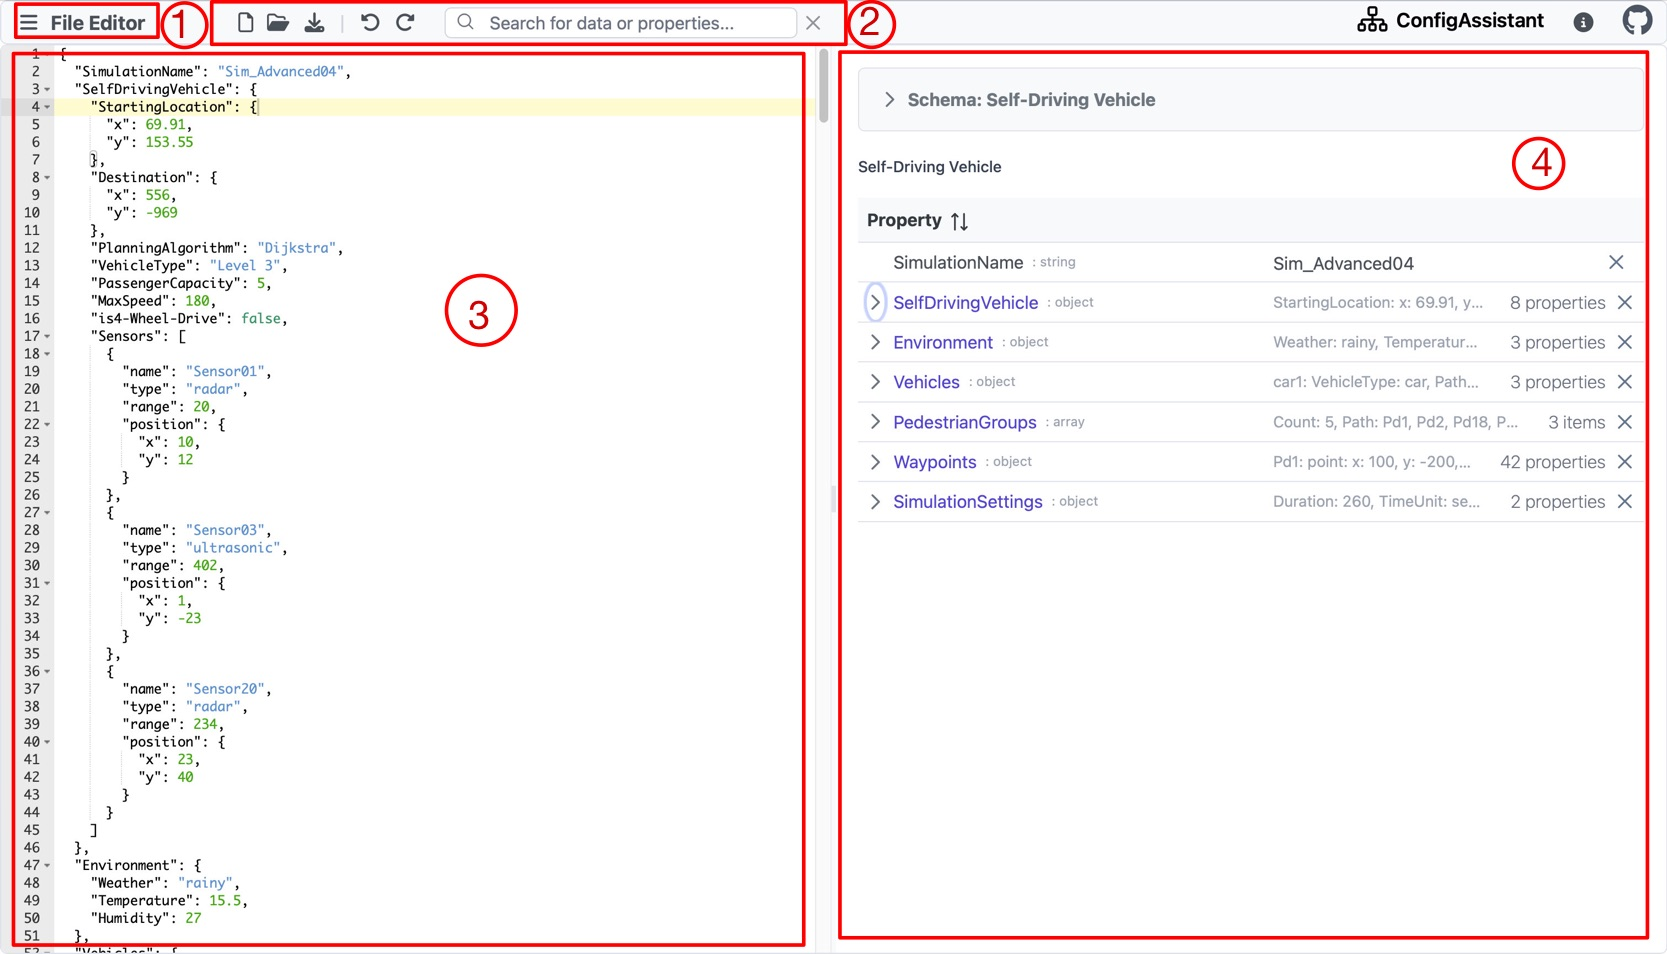
\includegraphics[width=\textwidth]{figures/fileeditor}
    \caption{FileEditor}
    \label{fig:fileeditor}
\end{figure*}

\begin{figure*}
    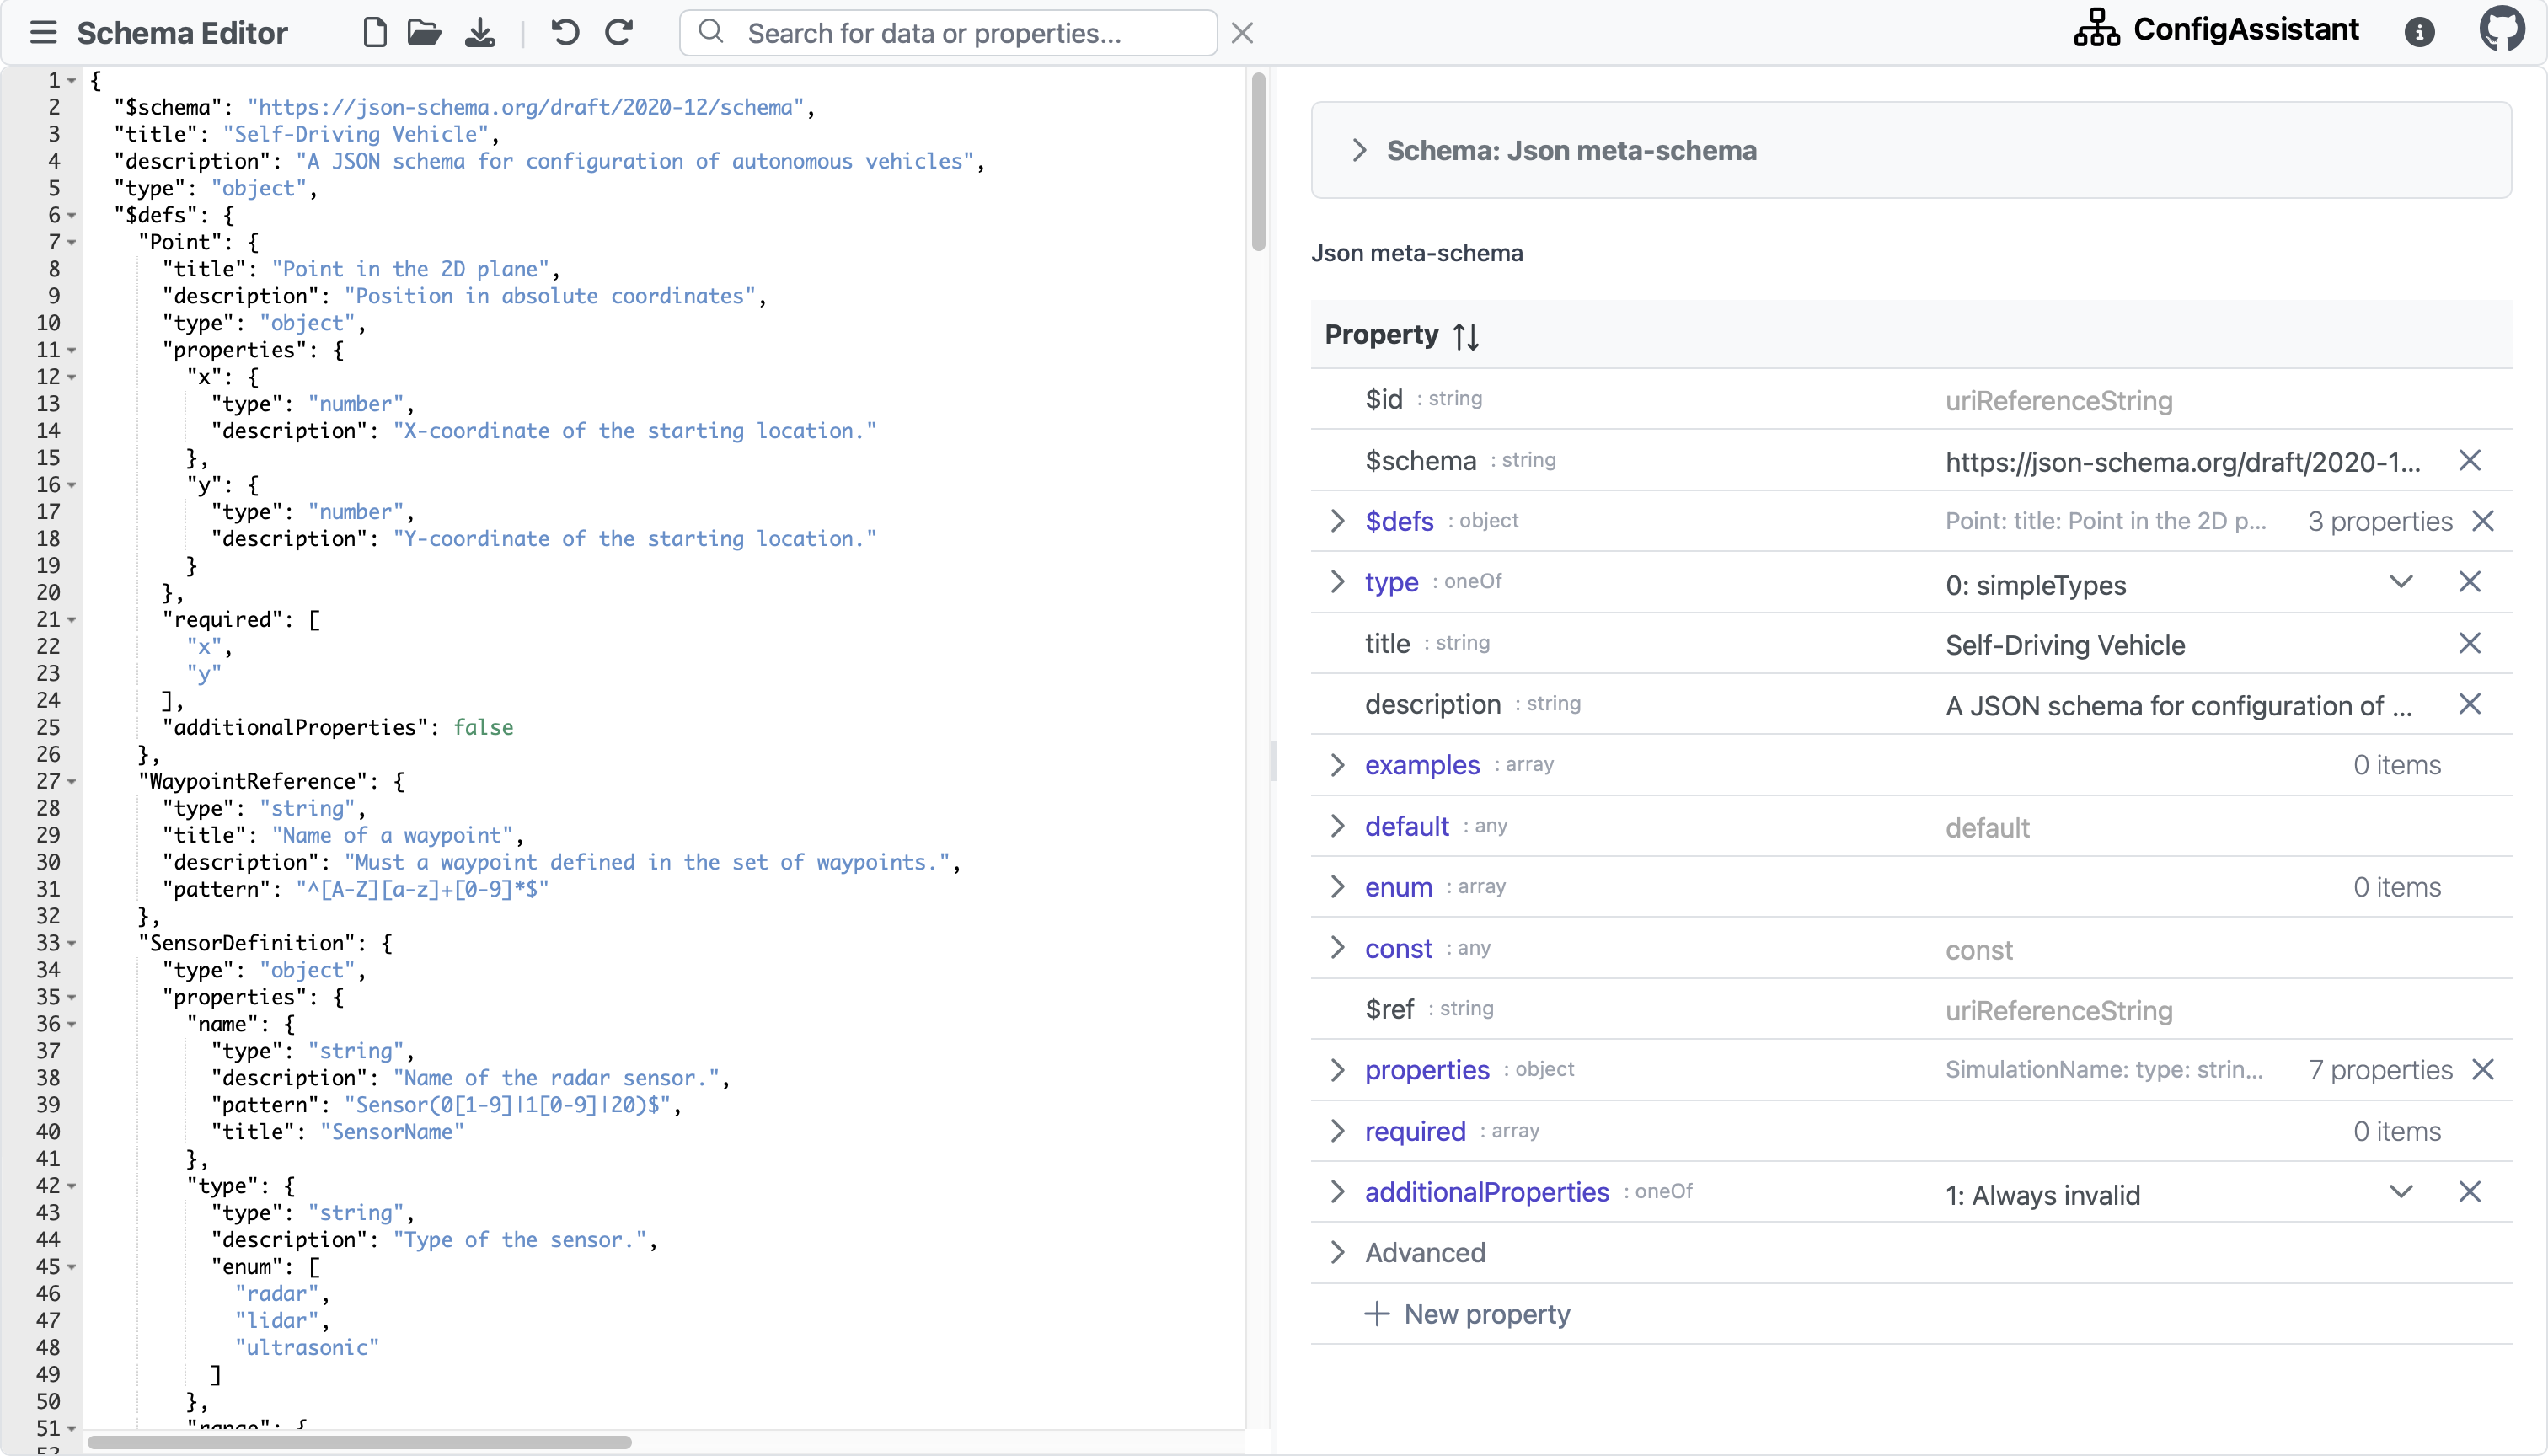
\includegraphics[width=\textwidth]{figures/schemaeditor}
    \caption{SchemaEditor}
    \label{fig:schemaeditor}
\end{figure*}

\begin{figure*}[h]
    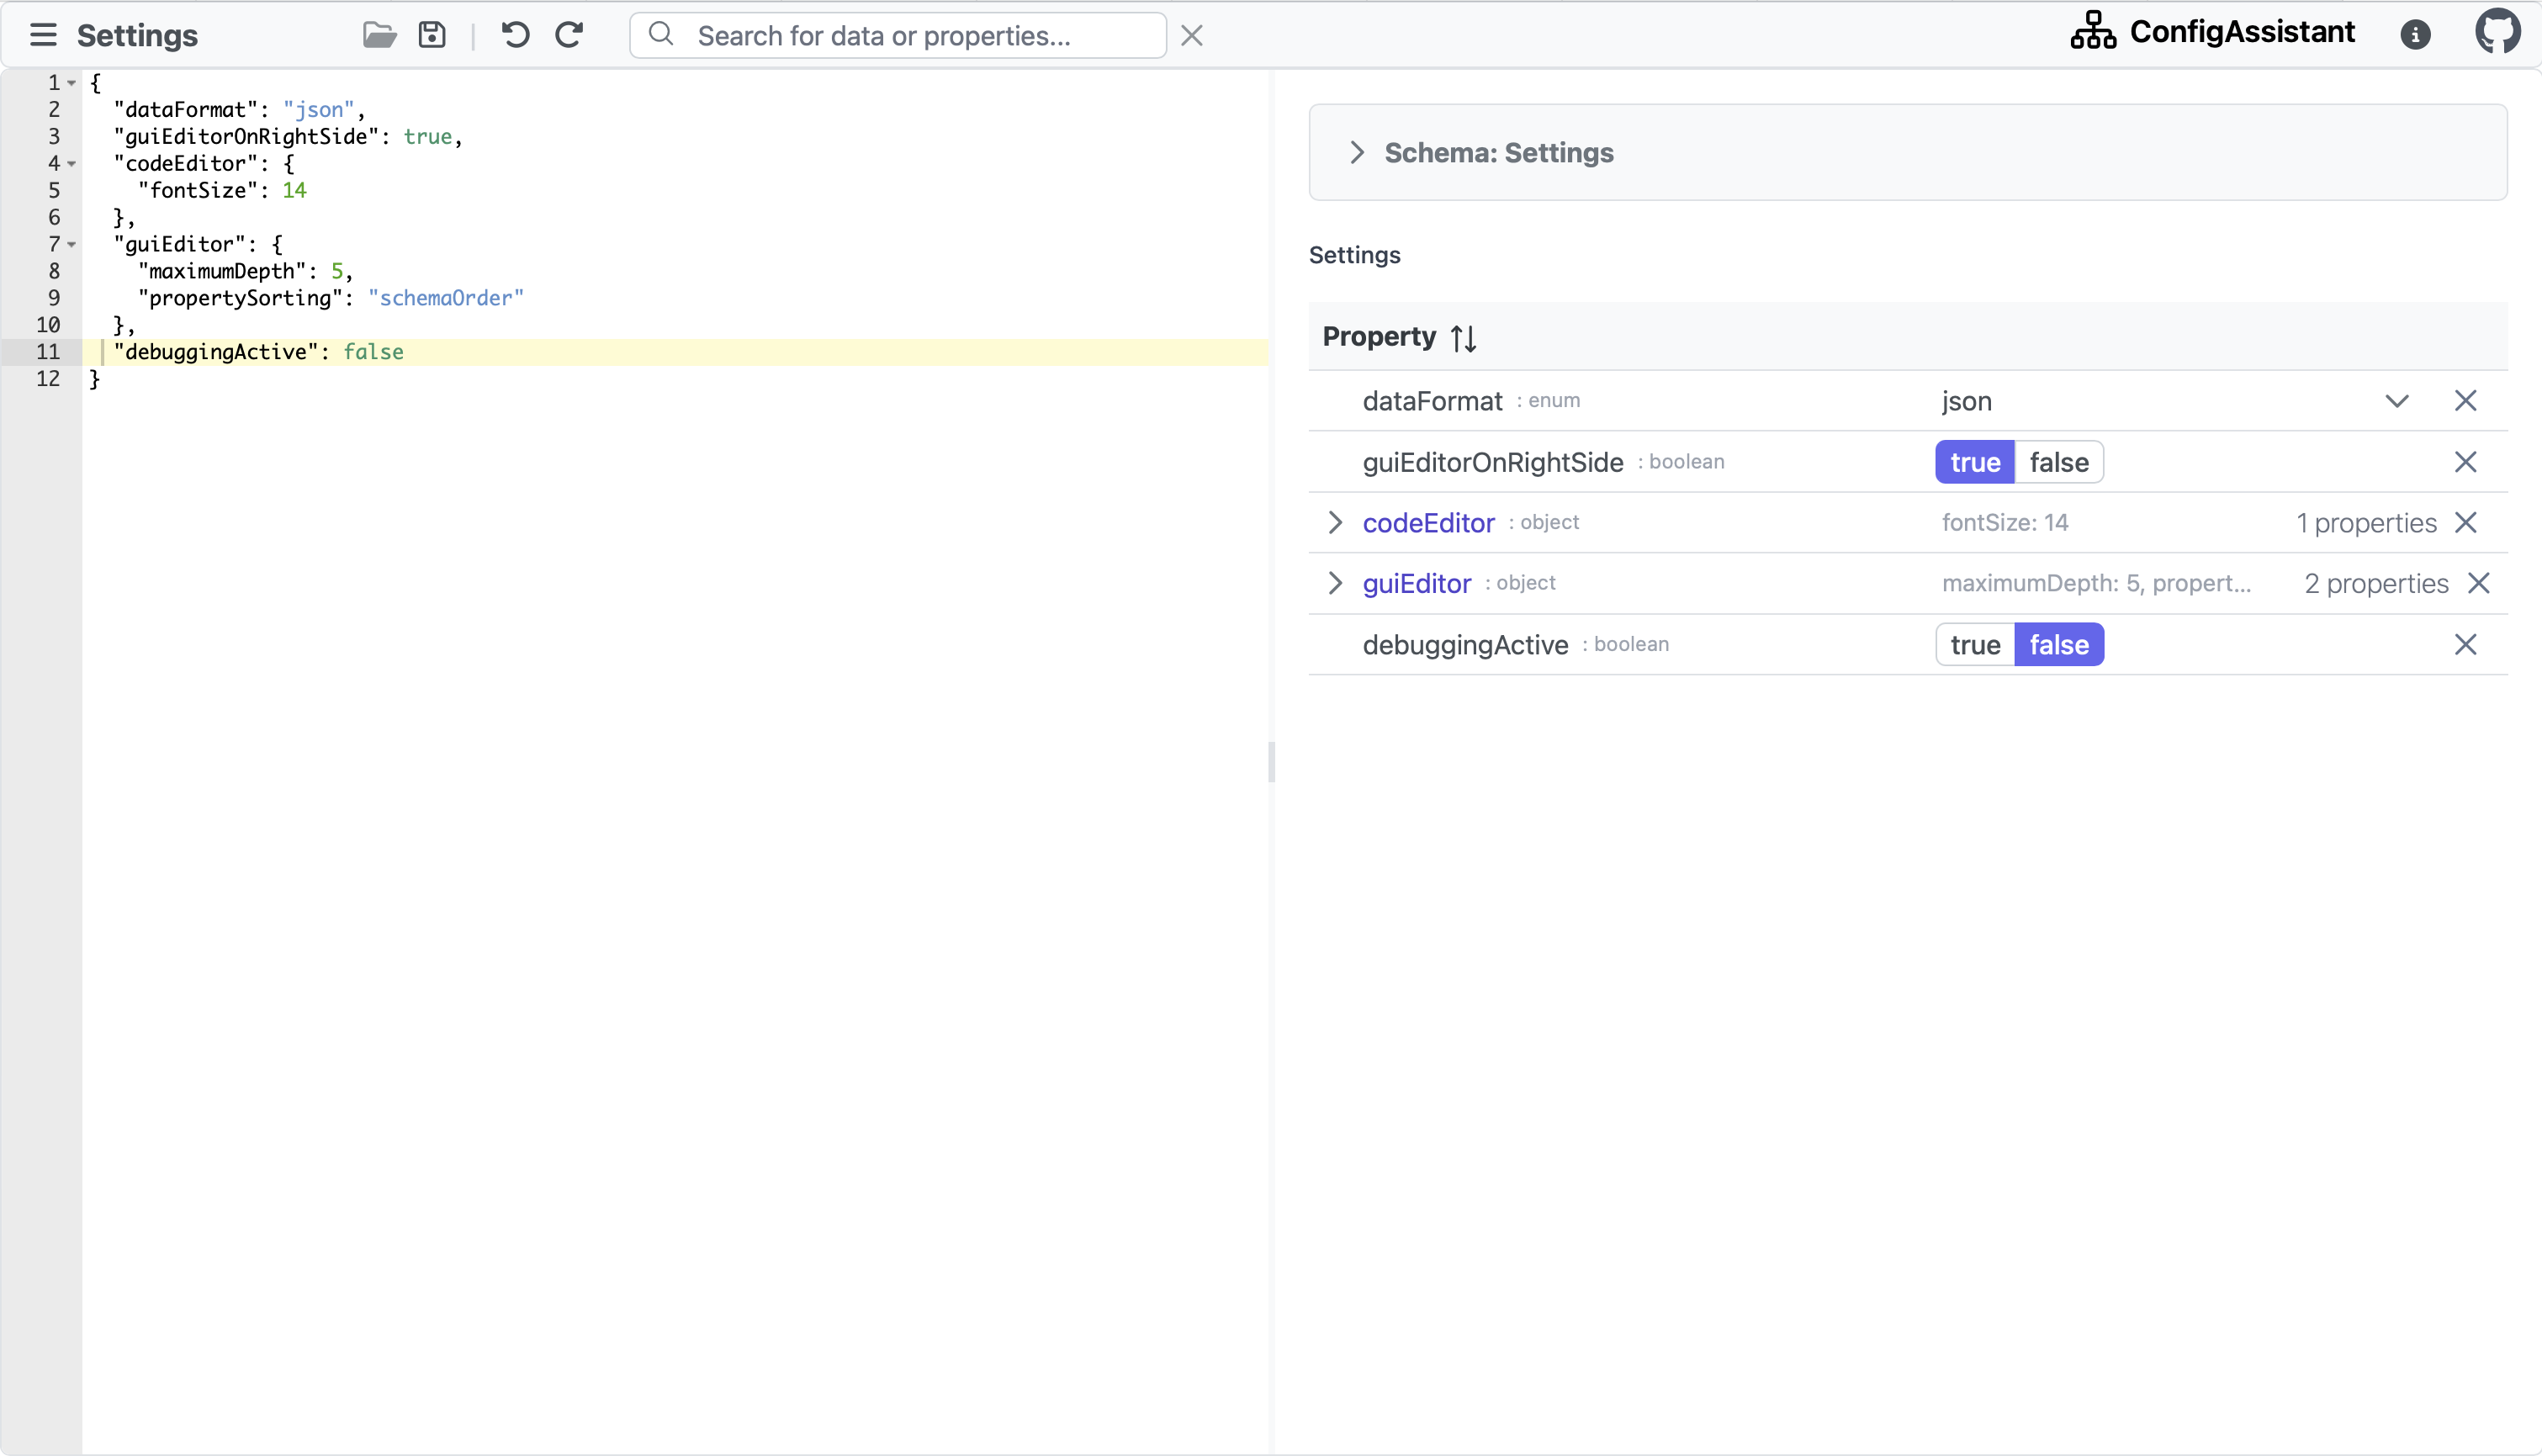
\includegraphics[width=\textwidth]{figures/settings}
    \caption{Settings}
    \label{fig:settings}
\end{figure*}

\subsubsection{Toolbar functionalities}

The toolbar provides basic functionalities for all three views:
\begin{itemize}
    \item \textbf{New File:} Create a new (schema) file.
    In the file editor, this option also includes two sub-items:
    \begin{itemize}
        \item \textbf{Generate Data:} Generate random configuration data based on the selected schema from the Schema Editor.
        \item \textbf{New Empty File:} Start with a blank file, discarding any current changes.
    \end{itemize}

    \item \textbf{Open File:} Open an existing file.
    For the File Editor, this opens a dialog to open a file from the local file system.
    For the Schema Editor, this comes with four sub-options:
    \begin{itemize}
        \item \textbf{JSON Schema Store:} Choose a schema from the JSON Schema Store, which provides a list of available schemas.

        \item \textbf{From Our Examples:} Access four example schemas provided within the tool.

        \item \textbf{From File:} Select a schema from local file system.

        \item \textbf{From URL:} Provide the URL of a specific schema, and the tool will retrieve and open it.

    \end{itemize}
    \item \textbf{Undo/Redo:} Undo or redo the latest operations in the editor.
    \item \textbf{Download:} Download the current editor content with an appropriate file name.
    \item \textbf{Search:} Text field where the user can enter a search term to find and navigate to specific sections within the current file.
\end{itemize}


\subsubsection{Settings}

In the Settings view (figure~\ref{fig:settings}), the user can adjust various parameters (tab~\ref{tab:settings})of \toolname{}:
\begin{table*}
    \centering
    \caption{Setting Parameters\label{tab:settings}}
    \begin{tabular}{@{}p{0.3\linewidth}p{0.6\linewidth}@{}}
        \toprule
        \textbf{Parameter} & \textbf{\ Description} \\
        \midrule
        Data Format & The data format used by the code editor. Currently YAML and JSON are supported. \\
        Code Editor Font Size & Size of the font in the code editor. \\
        Gui Editor On Right Side & By default, the GUI panel is located on the right side and the code panel on the left side. Using this option, their positions can be swapped. \\
        GUI Editor Property Sorting & The order in which the properties in the GUI panel should appear:
        \begin{itemize}
            \item \textbf{Schema Order}: Orders elements according to the order in the schema.
            \item \textbf{Priority Order}: Orders elements based on their priority (e.g. required properties first, deprecated properties last).
            \item \textbf{Data Order }: Orders elements the same way as it is in the data.
        \end{itemize} \\
        GUI Editor Maximum Depth & Determines the maximum level of nesting or hierarchy displayed in the GUI editor. \\
        Debugging Active & For debugging purposes, users can enable or disable the debugging panel as needed.  \\
        \bottomrule
    \end{tabular}
\end{table*}


\subsection{Code Panel}\label{subsec:code-editor}

The code editor is a GUI panel designed for editing the \cfgfiles.
For this project, we use the popular \textbf{Ace Editor}\cite{Ace-Editor} library to embed an interactive code editor into our user interface.
% It is a browser based editor that matches and extends the features, usability and performance of existing native editors such as TextMate, Vim or Eclipse.
% It can be easily embedded in any web page or JavaScript application.

\subsubsection{Features}

To make our code editor more user-friendly, we implemented several features, which are described in the following.

\paragraph{Schema Validation}
To provide the user feedback on whether their data is valid according to the provided schema, we perform schema validation.
We make use of the \textbf{Ajv JSON schema validator}\cite{ajv-validator} library, which supports the newest JSON schema draft 2020-12.
%Ajv firstly generates a fast validation function from the input schema.
If schema violations are found, the corresponding user data lines in the code editor will be marked with a red error hint, which also describes the violation.


\paragraph{Syntax Highlighting}
Ace Editor supports syntax highlighting for both JSON and YAML, which we use.
The data format can be switched in the \textit{Settings} page.
Note that Ace Editor allows to collapse/expand segments of the text, based on the hierarchical tree structure of the data.

\paragraph{Linkage of text with the data model}
As described in section \ref{subsubsec:design_text_editor_panel}, to map a cursor position in the text editor to a path in the data model we need to implement the function \textit{determinePath(editorContent, cursorPosition)} and to map a path in the data model to a text row in the editor, we need to implement the function \textit{determineRow(editorContent, dataPath)}. For every data format to be supported, those two functions need to be implemented.

For \textit{JSON}, the functions have been implemented using a \textit{Concrete Syntax Tree (CST)}.
The text content is parsed as a CST. Then the tree is is traversed recursively.
Every tree node has a range property, describing the start and end index of the text belonging to the node.
To determine the corresponding path for a cursor position, the cursor position is translated to a character index $targetCharacter$ within the text.
Then the CST is traversed and for all nodes $currentNode$ of type array or object for which $targetCharacter \in currentNode.range$,
the child nodes are checked and the key of the node (or index for array elements) is appended to the result path.
This way, the corresponding path is built up.
To determine the cursor position for a given path, the reverse is done: the CST is traversed until the effective path of the $currentNode$ is the target path. Then $currentNode.range.start$ is returned as result index, which is then translated into a cursor position (row and column).

% TODO: section for YAML.

\paragraph{Editor Operations}
The code editor has more functionalities, such as the possibility to open a file by drag and drop into the editor, as well as customizable font sizes.

\subsection{GUI Panel}\label{subsec:gui-editor}

The GUI editor is a component that allows the user to edit the configuration data in a GUI, which is generated based on the schema of the configuration data.
It is structured in a table-like way, where each row represents a key-value pair of the configuration data.
Arrays elements are represented similarly, where the index of the array element is the key and the value is the array element itself.
Figure~\ref{fig:gui-editor} shows the GUI editor component with an example schema and configuration data.

\begin{figure}[!t]
    \centering
    \includegraphics[width=\columnwidth]{figures/gui-editor} % todo replace with screenshot
    \caption{GUI Editor Component}
    \label{fig:gui-editor}
\end{figure}

To allow this representation of the schema, we do some preprocessing of the \textbf{schema}, which is described in section~\ref{subsec:schema-preprocessing}.

\subsubsection{Features}\label{subsubsec:gui-editor-features}

To assist the user in editing the configuration data, the GUI editor offers a set of features, which are described in the following.

\paragraph{Traversal of the Data Tree}
By default, only the first level of the data tree is shown.
The user can expand the data tree by clicking on the arrow next to the key of an object or array.
This will show the sub-properties of the object or the elements of the array.
We limit the depth of the data tree to a configurable value, to prevent the GUI editor becoming too overwhelming.
However, the user can also click on the property name or array index to \textit{zoom in} to that element.
This will show the sub-properties of that element at the top level, as if that property was the root of the data tree.
The breadcrumb at the top allows the user to see which path the GUI editor currently shows and to navigate back to upper levels of the tree.

% todo add figure to illustrate (for all the different data types and features)

\paragraph{Type specific components}

% todo write

\paragraph{Remove Data}
The user can delete properties or array elements from the data by clicking on the $\times$ button next to the edit field.
This button is only shown if the property is not required and there exists data.

\paragraph{Schema Information Tooltip}
When the user hovers over the property key or array index, an overlay is displayed, which contains all information from the schema about that property.
We manually implemented a generation of a textual description for each of the JSON schema keywords.
Starting with title and description of the property, the overlay then shows constraints (such as the number must be greater than 0) and in the bottom it also shows schema violations, in case there are any.
This feature helps the user to understand the constraints and the meaning of a property.

\paragraph{Highlighting Schema Validation Errors}
When the configuration data does not comply to the schema, the corresponding elements are underlined in red and highlighted with a red error icon.
This way, the user knows where any errors are.
Additionally, the schema information tooltip lists all schema violations.
% todo add screenshot

\subsection{Schema preprocessing}\label{subsec:schema-preprocessing}

To represent the schema in the GUI editor, we preprocess the schema.
We differentiate between three ways of preprocessing:
A one-time preprocessing step when loading the schema, an internal preprocessing that happens at every layer of the schema tree,
and calculating an effective schema that happens every time the configuration data changes.

\subsubsection{One-time Preprocessing Step}
When the schema is loaded, we perform a one-time preprocessing step that currently only involves migrating the schema to the newest version,
as described in section~\ref{subsec:json-schema-versions}.
The user will be informed about this step and also prompted with a dialog, when the schema file does not define which JSON schema version it uses.
After the migration, the resulting schema is loaded into the tool in the \textit{Schema Editor} page.

% todo maybe describe how bundling might make sense here

\subsubsection{Internal preprocessing}
This preprocessing steps are mainly used to generate the GUI editor and thus are internal steps that will not be visible for the user.
They happen at every layer of the schema tree lazily, only when required.
Laziness of the preprocessing is required as schemas can have circular references, which would, otherwise, lead to infinite loops.
In the following, we describe the preprocessing steps in details.

\paragraph{Resolving references}
JSON schema uses the \texttt{\$ref} keyword to reference other schemas.
This can either be references to schemas in the same file (using the \texttt{\$defs} keyword), references to other local files,
or references to schemas at a URL in the web.
We currently only support references to schemas in the same file.
These are lazily resolved as the first preprocessing step.
Listing~\ref{listing:preprocessing-example} shows an example schema, Listing~\ref{listing:reference-resolving} shows the equivalent example after
this first preprocessing step.

\begin{listing}[!h]
    \begin{minted}[frame=single,
        framesep=3mm,
        linenos=true,
        xleftmargin=15pt,
        tabsize=4]{json}
{
  "title": "NonEmptyString",
  "$ref": "#/$defs/nonEmptyString",
  "$defs": {
    "nonEmptyString": {
      "type": "string",
      "minLength": 1
     }
  }
}
    \end{minted}
    \caption{Simple JSON schema before reference resolving}
    \label{listing:preprocessing-example}
\end{listing}

\begin{listing}[!h]
    \begin{minted}[frame=single,
        framesep=3mm,
        linenos=true,
        xleftmargin=15pt,
        tabsize=4]{js}
{
  "allOf": [
   {
     "title": "NonEmptyString"
   },
   {
     "type": "string",
     "minLength": 1
   }
  ],
  "$defs": {
    "nonEmptyString": {
      "type": "string",
      "minLength": 1
     }
  }
}
    \end{minted}
    \caption{Simple JSON schema after reference resolving}
    \label{listing:reference-resolving}
\end{listing}

\paragraph{Resolving allOfs}

The \texttt{allOf} keyword in JSON schema specifies that all of the schemas in the given array must be valid.
To simplify any other operation on the schema, we aim to merge the schemas in the allOf array to one equivalent schema.
As the first step, we do a recursive step by preprocessing all the schemas of the allOf array.
Then, we use the \textit{mergeAllOfs} library % todo citation
for this task.
Listing~\ref{listing:resolved-allOf} shows the previous example schema after this step.
It is important to note that this library only supports a few keywords of JSON schema, most notably the
\texttt{properties} and \texttt{items} keyword.
Hence, the support for allOf and any other keywords for which we use this in the preprocessing is limited.

\begin{listing}[h]
    \begin{minted}[frame=single,
        framesep=3mm,
        linenos=true,
        xleftmargin=15pt,
        tabsize=4]{js}
{
  "title": "NonEmptyString"
  "type": "string",
  "minLength": 1,
  "$defs": {
    "nonEmptyString": {
      "type": "string",
      "minLength": 1
     }
  }
}
    \end{minted}
    \caption{Simple JSON schema after allOf resolving}
    \label{listing:resolved-allOf}
\end{listing}


\paragraph{Converting types to oneOf}
In JSON schema, a property can have multiple supported types, such as shown in listing \ref{listing:multiple_types}.
A semantically equivalent schema can be generated by the use of oneOf, where each sub-schema contains exactly one of the types, as shown in listing \ref{listing:multiple_types_converted}.
If a schema defines more than one type, we convert the types to oneOf. This way, we reduce complexity by having to solve only the problem of oneOf.
For schemas that already contain oneOf, every type is multiplied with every existing oneOf sub-schema.
For 2 types and 3 oneOf sub-schemas, this will result in a new oneOf with 6 options.
An exception is when a type can not be merged with an oneOf sub-schema (e.g. the type is "boolean" and the oneOf sub-schema has type "string").
In that case, the incompatible pair is dismissed.

\begin{listing}[!h]
    \begin{minted}[frame=single,
        framesep=3mm,
        linenos=true,
        xleftmargin=15pt,
        tabsize=4]{json}
{
  "type": ["object", "boolean"]
}
    \end{minted}
    \caption{Simple JSON schema with two possible types}
    \label{listing:multiple_types}
\end{listing}

\begin{listing}[!h]
    \begin{minted}[frame=single,
        framesep=3mm,
        linenos=true,
        xleftmargin=15pt,
        tabsize=4]{js}
{
  "oneOf": [
    {
      "type": "object"
    },
    {
      "type": "boolean"
    },
  ]
}

    \end{minted}

    \caption{Simple JSON schema after conversion of types to oneOf}
    \label{listing:multiple_types_converted}
\end{listing}


\paragraph{Removing incompatible oneOfs and anyOfs}
It can happen that a schema has oneOf or anyOf options which are not compatible with the schema of the property (e.g. sub-schemas that can never be fulfilled in combination with the property schema).
Listing \ref{listing:incompatible_one_ofs} provides an example of a schema with an incompatible oneOf option.
An example where this occurs is in our adjusted JSON schema meta schema, if we assign the root property the jsonSchema sub-schema, which allows objects and booleans, but then additionally restrict the root to be an object.
For every oneOf and anyOf sub-schema, we check whether it can be merged with the schema of the property.
The options which are not compatible (can not be merged) are removed (see listing \ref{listing:incompatible_one_ofs_removed}).

\begin{listing}[!h]
    \begin{minted}[frame=single,
        framesep=3mm,
        linenos=true,
        xleftmargin=15pt,
        tabsize=4]{js}
{
  "type": "object",
  "oneOf": [
    {
      "type": "object"
    },
    {
      "type": "boolean"
    },
  ]
}
    \end{minted}
    \caption{Simple JSON schema with incompatible oneOf option}
    \label{listing:incompatible_one_ofs}

\end{listing}


\begin{listing}[!h]
    \begin{minted}[frame=single,
        framesep=3mm,
        linenos=true,
        xleftmargin=15pt,
        tabsize=4]{js}
{
  "type": "object",
  "oneOf": [
    {
      "type": "object"
    }
  ]
}
    \end{minted}
    \caption{Simple JSON schema with incompatible oneOf option removed}
    \label{listing:incompatible_one_ofs_removed}
\end{listing}


\paragraph{Merging singular oneOfs and anyOfs}
Because of the previous pre-processing step, it can happen that for some oneOfs or anyOfs there remains only one compatible sub-schema left (see listing \ref{listing:incompatible_one_ofs_removed}).
If this is the case, the use oneOf/anyOf is redundant, as that singular sub-schema must be chosen implicitly.
Therefore, if there exists only one singular choice for oneOf/anyOf, we merge its sub-schema into the property schema and remove the use of oneOf/anyOf (see listing \ref{listing:singular_one_of_merged}).

\begin{listing}[!h]
    \begin{minted}[frame=single,
        framesep=3mm,
        linenos=true,
        xleftmargin=15pt,
        tabsize=4]{js}
{
  "type": "object"
}
    \end{minted}
    \caption{Simple JSON schema with singular oneOf merged into property schema}
    \label{listing:singular_one_of_merged}
\end{listing}


\paragraph{Attempting to merge oneOfs into anyOfs}
Schemas can use both anyOf and oneOf at the same time.
Especially after converting all types (when there is more than one type) to oneOf, it happens that a schema has oneOf options (typically for types) and simultaneously anyOf options.
The user will then have to select both an oneOf sub-schema, as well as an anyOf sub-schema in the GUI.
We observed a special scenario in the JSON meta schema, where the oneOf selection was always implicitly given by the anyOf selection.
For every single anyOf sub-schema, only one oneOf sub-schema was compatible.
In that scenario, we can merge the oneOfs into the anyOfs: for every anyOf sub-schema, we merge the one compatible oneOf sub-schema into it.
This is precisely what this pre-processing step does: if possible, the oneOf sub-schemas are merged into the anyOf sub-schemas and the oneOf property is removed from the schema.


\paragraph{Preprocessing oneOfs and anyOfs}
For all remaining oneOf and anyOf sub-schems, the internal pre-processing steps are executed.


\paragraph{Title inducing}

The \texttt{title} keyword is used to give a schema a short description.
This is not necessarily the same as the property name of properties of an object.
As we use the title in various cases to display for the user, we inject the property name in cases where no explicit title is given.

\begin{listing}[!h]
    \begin{minted}[frame=single,
        framesep=3mm,
        linenos=true,
        xleftmargin=15pt,
        tabsize=4]{js}
{
  "type": "object",
  "properties": {
    "name": {
      "type": "string"
    }
  }
}
    \end{minted}
    \caption{Simple JSON schema with one property without a title}
    \label{listing:no-title}
\end{listing}

\begin{listing}[!h]
    \begin{minted}[frame=single,
        framesep=3mm,
        linenos=true,
        xleftmargin=15pt,
        tabsize=4]{js}
{
  "type": "object",
  "properties": {
    "name": {
      "title": "name",
      "type": "string"
    }
  }
}
    \end{minted}
    \caption{The property names was used for the title field}
    \label{listing:with-title}
\end{listing}

\paragraph{Processing enum and const}
The enum keyword is used to restrict the values of a field to a fixed set of valid values.
The const keyword, similarly, restricts the property value to a single allowed value.
Thus, setting the const value is equivalent to settings the enum value with an array that contains this single value.

We convert any usage of const to enums with a single element, which allows us to ignore the const keyword in other operations.

\subsubsection{Calculating an effective schema}

This third preprocessing step is calculated the most often, namely every time the data changes.
However, for most schemas this preprocessing step is trivial.
The JSON schema keywords \texttt{if}, \texttt{then}, and \texttt{else} provide a way to include conditions in the JSON schema.
If the schema in the \texttt{if} field is valid, then also the schema in the \texttt{then} field must be valid, otherwise the
schema in the \texttt{else} field must be valid.

This makes the schema data dependent.
To show the correct properties, we evaluate the data and dependent on validity or not, we either use the \texttt{then} or the \texttt{else} schema.

We similarly handle the \texttt{dependentRequired} and the \texttt{dependentSchemas} keywords.
For schemas without any of those keywords, this step is trivial as the schema is not modified in any way.

%todo examples

\subsection{Schema editor}\label{subsec:schema-editor}

The schema editor page has the same structure as the File editor page, as discussed in previous sections.
The only difference is that the schema used for generating the GUI panel is not the schema file provided by the user but the Json schema meta schema,
i.e., the schema that defines the structure of valid JSON schema files.
However, applying our generic approach on the official Json schema meta schema (TODO citation) does not result in a user-friendly editor for
creating and modifying schema files.
In this section we discuss the reasons for that and how we developed a new meta schema that circumvents the problems of the official meta schema.

\subsubsection{Missing descriptions}
With the \texttt{description} keyword, schema authors can give descriptions to any elements of their schema.
This can help the user of a schema in many ways, for example, the author can specify the unit of a numeric field or give other additional information.
The JSON schema meta schema does not provide any descriptions.
Users, especially those without prior knowledge in JSON schema, might not understand the meaning of the fields of JSON schema.
Thus, we insert descriptions from the JSON schema specification (TODO citation) into our modified meta-schema.

\subsubsection{External references}
\toolname does not support references to external schemas yet, i.e., references inside the schema to a schema at a specific URL\@.
Also, \toolname does not support the \texttt{\$vocabulary} keyword yet.
Both features are used in the JSON schema meta schema, as it is distributed over multiple schema files.
To circumvent that problem, we put all schemas in one schema file into the \texttt{\$defs} object and replace the external references with local references.

\subsubsection{Use of dynamic anchors and references}
The JSON schema meta schema uses dynamic references and dynamic anchors.
The difference of those keywords in comparison to the \texttt{\$ref} keyword is that they provide a way to dynamically extend the JSON meta schema
at runtime.
For example, one could combine the JSON schema meta schema with an extension that defines how fields should be serialized in XML\@.
We do not support dynamic references and anchors yet.
We replaced all of them by ``non-dynamic'' references using the \texttt{\$ref} keyword.

\subsubsection{Allowing each field in each context}
The JSON schema meta schema allows each field in each context.
For example, if the \texttt{type} keyword is used and set to \texttt{string}, then the \texttt{properties} keyword is allowed,
even though it does not make sense in that context.
According to the specification, any validator should ignore the fields that do not make sense in the current context.
Consequently, the user does not need to see those fields, but instead, the user gets overwhelmed by the amount of fields
and does not know which fields are relevant for the current context.
This is also a feedback we got from our user study.
Thus, we added \texttt{if} conditions to each field to only show them when they make sense in the current context.
Listing~\ref{lst:if-then-else} shows an example of such an \texttt{if} condition.
The relevant properties for arrays are only shown when the current property is of type array.

\begin{listing}[!h]
    \begin{minted}[frame=single,
        framesep=3mm,
        linenos=true,
        xleftmargin=15pt,
        tabsize=4]{json}
{
  "if": {
    "$ref": "#/$defs/hasTypeArray"
  },
  "then": {
    "$ref": "#/$defs/arrayProperty"
  }
}
    \end{minted}
    \caption{If condition for array properties. The \texttt{hasTypeArray} is valid if the current property is of type array. The \texttt{arrayProperty} schema defines the properties of an array.}
    \label{lst:if-then-else}
\end{listing}

To even more reduce the amount of fields shown to the user, we also introduced a custom keyword just for our own meta schema.
The keyword \texttt{advanced} is a boolean field that is set to \texttt{false} by default.
It is wrapped in an \texttt{metaConfigurator} object, which is ignored by any validator as it is not part of the JSON schema specification.
We use this wrapper to prevent any other schema extensions from colliding with our keyword.
When set to \texttt{true}, the field not shown by default, but only when the user expands the advanced section.
We put all fields that are not required for the basic usage of the schema into the advanced section.
For this, we oriented ourselves on the work of Baazizi et al.~\cite{baazizi2021empirical}, which analyzed the usage of JSON schema keywords in 82,000 JSON schemas.

% TODO screenshots


% paul
% todo consider putting somewhere else
\subsection{JSON schema versions}\label{subsec:json-schema-versions}

JSON schema has had 10 different drafts over the years, the newest being draft 2020--12~\cite{jsonschemaJSONSchema}.
In real-world we cannot expect all schemas to have the newest version.
Baazizi et al.~\cite{baazizi2021empirical} investigated over 82.000 open-source schemas in 2021, where they found that most of them are using draft 4, which was released in 2013.
As the different drafts are not necessarily compatible with each other, tools supporting one draft become outdated when a new draft releases.
However, Viotto et al.~\cite{Viotti_Lagoni_2023} provide a library for migration schemas from older versions to the newest draft without loss of information.
Thus, by using this library, our tool only needs to support the newest draft directly.
If a user uses a schema from an older draft, we first migrate it to the newest draft internally.


 \section{User Study}\label{sec:user_study}
 We conduct several interviews with professors and students as potential customers.
During each interview, we introduce \toolname{}, give the participant tasks to execute using the tool and finish the session with open ended questions. 
We observe how the participants work with the tool and which difficulties they have when executing the tasks.
Additionally, we ask them for feedback and improvement suggestions.
We also conduct a survey to gather demographic information about the participants of the user study.

Note that besides the user study we have applied \toolname{} on several schemas (such as EnzymeML\cite{TODO} and the Strenda schema\cite{TODO}, provided by professors that we worked with) and \cfgfiles{} from the real world, to verify that it works and does bring benefits to the user. 

\subsection{Methodology}\label{subsec:methodology}

\paragraph{Potential Users}
We look for potential users to conduct the interviews.
There are two basic standards we follow to find a potential user:
\begin{itemize}
    \item Professors and students who are interested in our application.
    \item People who frequently use \cfgfiles and schema languages
\end{itemize}

\paragraph{Interview Questions}
For the interview, we created a JSON schema and \cfgfile{}, about a made-up self-driving car simulation.
The interview questions deal with working with those files.
We divide our interview tasks into four parts:
\begin{itemize}
    \item Setup: Open the application and open schema and \cfgfile.
    \item Information Retrieval Questions: with increasing difficulty, the participant has to retrieve information from the \cfgfile{}. Much easier to solve by using the GUI panel.
    \item Configuration Modifications: Different tasks that involve changing the \cfgfile{}. Intend is that the participant becomes more familiar with the GUI panel.
    \item Schema modifications: Making adjustments to the schema. Most difficult, but still feasible using the GUI panel.
\end{itemize}

%TODO: include interview material in appendix

\paragraph{Interview Process}
We proceed our interview with one interviewee each time.
The interview lasts around one hour.
At the beginning, the interviewee is asked about approval of recording, and they can stop participating at any time.
We introduce \toolname{} to the interviewee. 
Then we send the participant the tasks and \cfgfile{} and let them work on the tasks while sharing their screen.
During this task solving session, we provide the interviewee with some basic help if they ask specific questions about the tool.
The interview is recorded and we make notes of the answers, feedback and behavior of the interviewee.e
Finally, in an open dialog, we ask the interviewee about more feedback and improvement suggestions as well as their opinion on the tool.

\paragraph{Survey}
After the interview, we ask each interviewee to fill out a survey (follow-up questions).
This survey covers the following points:
\begin{itemize}
    \item Occupation of the interviewee.
    \item Experiences in software engineering,
    \item Frequency of working with JSON/YAML files.
    \item Domains in which people use with JSON/YAML files.
    \item Feedback about the application after interview.
\end{itemize}
%Based on the survey, we could get many feedbacks which we can use in the future.
%We analyse the results which we get from the survey and improve our application afterward.

\subsection{Results}
We performed the user study on 5 participants.

\subsubsection{Task Results}
Table \ref{table:Results} shows the accuracy and difficulties that the participants had when solving the tasks.
Accuracy is determined as the ratio of tasks that were solved correctly without the need of any hints to the total number of tasks.
With the help of hints, all tasks could be completed by every participant.

\begin{table*}[]
    \label{table:Results}
    \begin{tabular}{|c|l|l|l|}
        \hline

        \multicolumn{1}{|l|}{} &
            \begin{tabular}[c]{@{}l@{}}
                Participant\\ Background
            \end{tabular} &

        \multicolumn{1}{c|}{
            \begin{tabular}[c]{@{}c@{}}
                Accuracy\\ \&\\ Notes
            \end{tabular}} &
        \multicolumn{1}{c|}{
            \begin{tabular}[c]{@{}c@{}}
                Biggest\\ Difficulties
            \end{tabular}} \\ \hline

        User Study 1 &
        \begin{tabular}[c]{@{}l@{}}
            Computer Science %Professor.
        \end{tabular} &

        \begin{tabular}[c]{@{}l@{}}
            Accuracy: 100\%(11/11)\\
            1. Effectively solved tasks\\ with help of tooltip\\
            2. All questions right
        \end{tabular} &

        \begin{tabular}[c]{@{}l@{}}
            Task 3.2: Setting Vehicle Type to highest level\\
            - Took some time to find the field; \\
            - Not used the search function
        \end{tabular} \\ \hline

        User Study 2 &
        \begin{tabular}[c]{@{}l@{}}
            Bioinformatics %Professor.
        \end{tabular} &

        \begin{tabular}[c]{@{}l@{}}
            Accuracy: 91\%(10/11)\\
            1. Found search function\\  to solve task\\
            2. Used both GUI and code editor\\ to solve tasks
        \end{tabular} &

        \begin{tabular}[c]{@{}l@{}}
            Task 4.2: Adding new property\\
            - Could not find where to add new property\\ in Schema Editor\\
            - Did not know how to edit property name
        \end{tabular} \\ \hline

        User Study 3 &
        \multicolumn{1}{c|}{Biochemistry, Biology} &
        \begin{tabular}[c]{@{}l@{}}
            Accuracy: 82\%(9/11)\\
            1. Solved questions effectively \\ using tooltip\\
            2. Not familiar with JSON,\\ but could still solve tasks with \\ some help
        \end{tabular} &

        \begin{tabular}[c]{@{}l@{}}
            Task 2.3: Duration of Simulation\\
            - Did not know one can use GUI panel \\    at the beginning\\
            Task 2.4: Valid humidity error\\ - Could not find invalidity of humidity\\
            - Ignored the error hint at beginning\\
            Task 4.2 Add new property\\  - Set property name in wrong place
        \end{tabular} \\ \hline

        User Study 4 &
        \begin{tabular}[c]{@{}l@{}}
            Already familiar with \\ JSON Schema
        \end{tabular} &

        \begin{tabular}[c]{@{}l@{}}
            Accuracy: 82\%(9/11)\\
            1. Added new property quickly\\
            2. Resolved all tasks rightly
        \end{tabular} &

        \begin{tabular}[c]{@{}l@{}}
            Task 2.4: Valid value of humidity\\
            - Did not find value was invalid\\
            - Did not find that he could use tooltip\\
            Task 3.2: Setting Vehicle Type to highest level \\
            - Not scrolling down in enum property\\
            Task 3.3: Validation Errors\\
            - Tried to find validation errors in schema editor\\
            - Thought red underline was spell checking
        \end{tabular} \\ \hline

        User Study 5 &
        \begin{tabular}[c]{@{}l@{}}
            Seldom worked with\\ JSON schema
        \end{tabular} &

        \begin{tabular}[c]{@{}l@{}}
            Accuracy: 100\%(11/11)\\
            1. Understood the tool very well\\
            2. Quickly found all errors\\     and solved them\\
            3. Knew to use both GUI \\and code editor of tool
        \end{tabular} &

        \begin{tabular}[c]{@{}l@{}}
            Task 3.2: \\  - Took some time to find the vehicle type\\
            Task 4.2: Adding new property\\  - Did not set the property type at the beginning
        \end{tabular} \\ \hline
    \end{tabular}
    \caption{Results}
    \label{tab:my-table}
\end{table*}

\subsubsection{Feedback and Resolution} %Keyuri
Tables \ref{tab:user_study1}-\ref{tab:user_study5} show the feedback of the interviewees, as well as which measures we took based on it.

\begin{table*}
    \vspace{-10pt}
    \centering
    \small % Reduce font size
    \setlength{\extrarowheight}{5pt} % Add extra vertical space
    \renewcommand{\arraystretch}{1.5} % Adjust the vertical spacing between rows
    \begin{tabular}{|c|p{0.4\linewidth}|p{0.4\linewidth}|}
        \hline
        \multicolumn{1}{|c|}{} & \multicolumn{1}{|c|}{Feedback} & \multicolumn{1}{|c|}{Resolution} \\
        \cline{2-3}
        \hline
        User Study 1 & The property value should not be autocorrected if the user enters an incorrect value. 
        Instead, an error message or another way should be used to inform the user that their input is incorrect. & 
        Instead of auto-correcting values, we now provide more clear user feedback on incorrect values (red underline, error symbol). \\
        \cline{2-3}
        & It would be good to have the ability to remove data entries with the GUI panel. & 
        Implemented by adding a "remove" button next to properties which have data and are not required. \\
        \cline{2-3}
        & A search functionality to locate properties would be helpful, especially within nested levels.
        & Implemented in the toolbar. All findings are highlighted in the GUI panel. \\
        \cline{2-3}
        %& 4. The Schema editor GUI panel contains extensive metadata, but the code editor panel remains empty. & 4. bla bla bla \\
        \cline{2-3}
        & The GUI panel feels overwhelming to the user due to many variations in styling and color of the GUI elements. & 
        We slightly reduced the number of different stylings by no longer showing required properties in bold face and instead just show an asterisk next to it. \\
        \cline{2-3}
        & The cursor should not have the clickable animation when hovering over non-clickable fields in the GUI editor. & Now we only show the clickable animation when hovering over clickable GUI components. \\
        \cline{2-3}
        & In drop-down menus we do not need a button to clear the selection. & 
        We disabled the option of clearing the selection. \\
        \cline{2-3}
        & 8. If the type of a property is "any", it should not be interpreted as the "string" type in the GUI panel. & 
        We show a drop-down menu to the user, where they can select the type they want to use. \\
        \cline{2-3}
        & Validation errors should not highlighted via a warning symbol, but instead an error symbol & 
        We changed the warning symbol into an error symbol. \\
        \cline{2-3}
        & After performing an undo or redo action, the cursor should jump to the corresponding location to reflect the changes made by the user.& 
        Will be considered in future work. \\
        \hline
    \end{tabular}
    \caption* {User Study Feedback and Resolution (Continued)} \label{tab:user_study1}
\end{table*}


\clearpage % Force a page break

\begin{table*}

    \centering
    \small % Reduce font size
    \setlength{\extrarowheight}{5pt} % Add extra vertical space
    \renewcommand{\arraystretch}{1.5} % Adjust the vertical spacing between rows
    \begin{tabular}{|c|p{0.4\linewidth}|p{0.4\linewidth}|}
        \hline
        User Study 2 & A graph-based view would be more intuitive for handling complex data structures. & 
        Will be considered in future work. \\
        \cline{2-3}
        & Providing immediate feedback to users when they enter incorrect ranges is essential to prevent them from inputting invalid values into the property. & 
        We now highlight schema violations by a red error symbol in the GUI panel and underlining the property name in red. 
        Additionally, the tooltip lists all schema violations of a property. \\
        \cline{2-3}
        & Validation errors should also be reflected in the GUI panel, including for child properties. & 
        See point above. 
        Also, now the tooltip lists schema violations of child properties. \\
        \cline{2-3}
        & When dealing with an array, the display name of array elements (index) should be improved.
        Currently you show just the element index. & 
        We replace the numerical labels by a standard programming notation, which is \texttt{propertyName[0]}, \texttt{propertyName[1]}, ...
        \\
        \cline{2-3}
        & The input field next to the \textit{Add Item} button is confusing. Both the input field and the button can be used to create a new item, which is redundant.
        & We removed the input field next to the button. \\
        \cline{2-3}
        & It would be more consistent, if all user input in the GUI panel was within the right column of the table. 
        That in some scenarios user input is needed within the left column (for names of new properties) feels inconsistent.
         & Because of the nature of JSON schema, we retained the property name within the left column. 
         To make it clear to the user that the property name can be edited, we added an \textit{edit} icon next to it. \\
        \cline{2-3}
        & The search function for locating specific properties lacks clarity at first glance. 
        It should provide an immediate response and extend to nested levels, rather than merely highlighting the higher-level findings. & 
        The search now provides a list of results, and upon clicking on a particular result, it jumps to that result in the code panel and GUI panel. In the GUI panel, if the element is nested, its parents will be automatically expanded. \\
        \hline
    \end{tabular}
    \caption*{User Study Feedback and Resolution (Continued)} \label{tab:user_study2}

\end{table*}

\begin{table*}
    \centering
    \small % Reduce font size
    \setlength{\extrarowheight}{5pt} % Add extra vertical space
    \renewcommand{\arraystretch}{1.5} % Adjust the vertical spacing between rows
    \begin{tabular}{|c|p{0.4\linewidth}|p{0.4\linewidth}|}
        \hline
        User Study 3 & Working with the schema editor is difficult for me. It does not feel intuitive. & 
        We made the schema editor more intuitive by creating our own simplified JSON schema meta schema.
        For example, advanced JSON schema features are separated from the simple ones.
        See section TODO \\
        %% TODO
        \cline{2-3}

        \hline
    \end{tabular}
    \caption*{User Study Feedback and Resolution (Continued)} \label{tab:user_study3}

\end{table*}

\begin{table*}

    \centering
    \small % Reduce font size
    \setlength{\extrarowheight}{5pt} % Add extra vertical space
    \renewcommand{\arraystretch}{1.5} % Adjust the vertical spacing between rows
    \begin{tabular}{|c|p{0.4\linewidth}|p{0.4\linewidth}|}
        \hline
        User Study 4 & Modifying or renaming a new property in the GUI panel does not appear to take effect when double-clicking on it. & 
        Renaming properties in the GUI panel can now be done using the \textit{edit} button next to the property name. \\
        \cline{2-3}
        & When creating a new property in the schema editor, its sub-schema has to be selected, such as \textit{string property} or \textit{boolean property}. 
        Additionally, the type of the property has to be selected by the user too. 
        Therefore, for example, when creating a new \textit{string property}, the user has to select that it is a string two times. 
        It would be much more intuitive if the selection needs to be done only one time.  
        & We completely overhauled our JSON schema meta schema. 
        Now, when creating a new property, the user will have to select the type only once. \\
        \cline{2-3}
        & A toggle button should be implemented to enable and disable the code panel and GUI panel. 
        & Only having a GUI panel or only having a code panel restricts the user unnecessarily.
        The interplay of both panels is what makes this tool most effective.
         If the user does not want to use one of the panels, he can resize that panel to a very small size.  \\
        \cline{2-3}
        & When working with a particular property in the GUI panel the opacity of the other properties should be decreased, visually highlighting the property that currently is in focus. & Will be considered in future work. \\
        \cline{2-3}
        & 5. Simply the schema editor to make it easier to work with, for those who are not very familiar with JSON schema. &
        Has been done. See TODO. \\
        % TODO
        \hline

    \end{tabular}
    \caption{User Study Feedback and Resolution (Continued)} \label{tab:user_study4}

\end{table*}

\begin{table*}

    \centering
    \small % Reduce font size
    \setlength{\extrarowheight}{5pt} % Add extra vertical space
    \renewcommand{\arraystretch}{1.5} % Adjust the vertical spacing between rows
    \begin{tabular}{|c|p{0.4\linewidth}|p{0.4\linewidth}|}
        \hline
        User Study 5 & The search button is not immediately evident, making it challenging for users to locate the search function. & 
        Instead of showing the search bar only when clicking the search button, we now just always show it. \\
        \hline

    \end{tabular}
    \caption{User Study Feedback and Resolution (Continued)} \label{tab:user_study5}

\end{table*}



% TODO: if some quantitative methods are found, also mention here


 \section{Discussion}\label{sec:discussion} %Paul

 This section discusses the implications of our work and future work.


\subsection{Implications of our work}\label{subsec:implications-of-our-work}

\toolname{} provides a novel approach for editing \cfgfiles{}
by combining the advantages of a GUI and a code editor
Our user study suggests that \toolname{} is easy to use and intuitive and
that it has practical use cases in many domains.
However, the user study also revealed some limitations of \toolname{}.
Editing schemas with \toolname{} is not as intuitive as editing \cfgfiles{},
especially for users who are not familiar with JSON schema.
JSON schema may be feature-rich and expressive, but it is also complex and
hard to understand for new users.
%Specialized editors for schemas, such as those discussed in section~\ref{subsubsec:schema-editors},
%may be more suitable for this task.

\subsection{Future work}\label{subsec:future-work}
To make \toolname{} more useful for users who are not familiar with JSON schema,
there are several possible improvements.
First, a visual schema editor could be added to \toolname{}, similar to schema editors
discussed in section~\ref{subsubsec:schema-editors}.
These would provide a graph view of the schema, which is easier to understand than
the JSON schema in text form or the tree view in \toolname{}.
Second, \toolname{} could provide more guidance for users who are not familiar with JSON schema,
e.g., by providing an interactive tutorial or supporting a less complex schema language.

There are many other possible improvements to \toolname{}.
A desktop version of \toolname{} could be developed, which would allow users to
edit files on their local machine, which is more convenient than loading them into the web application.
Similarly, integration in other tools, such as IDEs, could be helpful for many users.
\toolname{} currently only supports JSON schema draft 2020--12, but it could be extended to support
other drafts by converting imported schemas to the latest draft.
Furthermore, YAML is not fully supported yet, which could be added in the future.
Another point that can be addressed is the loss of formatting and comments in YAML documents, when they are updated with new data.
This could be avoided by replacing only the section in the YAML document that corresponds to the change, instead of replacing the complete document.
To allow for different styles of formatting, the user could be provided with global formatting style settings (such as level of indentation or whether in YAML strings should be in quotation marks or not).
To deal with the loss of comments, a technique that keeps track of any comments in the text and then restores them after the text is replaced could be implemented. This has already been done in another tool of one of the authors\cite{githubBspEditor}.

Finally, \toolname{} could be extended to support code generation, e.g., for generating
Java classes from a JSON schema, which is useful for developers.

To improve the user study, it could be repeated with more participants,
so that the results are more representative.
Instead of just having participants solve tasks, it could also be interesting to
have one group of participants solve tasks with \toolname{} and another group solve
the same tasks with only a text editor.
This way, we could evaluate whether \toolname{} is actually more efficient than
just using a text editor.




 \section{Conclusion}\label{sec:conclusion} % Felix

%This paper addresses the challenge of managing and modifying \cfgfiles{} by introducing \toolname{}, a tool that provides a GUI for editing \cfgfiles{} based on a given schema.
% According to the criteria expressiveness and popularity, we choose JSON schema as schema format for the tool.
 This paper addresses the development of \toolname{}, a tool that generates YAML/JSON file editor GUIs tailored to a given data schema.
Our approach allows users to edit \cfgfiles{} in a GUI, while still having the flexibility and speed of a code editor.
Additionally, it removes the need for developing and maintaining a custom GUI for a particular schema.
We use JSON schema as a schema language for the tool as it is an expressive and popular schema language.
The tool is successfully implemented and our user study shows that it can be applied to solve practical tasks in 1) retrieving information from \cfgfiles{} in the context of a schema, in 2) modifying \cfgfiles{}, and in 3) editing schemas.
The interest and positive feedback of the participants suggests that \toolname{} will be used in practice.

% The text below is more suitable for a summary
%We evaluate existing schema languages by expressiveness and popularity and choose JSON schema as the most suitable for this work.
%We created a mockup showing how the tool should look like and designed the architecture, with modularity being one of the key aspects.
%For example, data formats (JSON/YAML/XML) or the different panels (GUI/rich text code editor) can be seen as building blocks that are exchangeable.
%We implemented \toolname{} according to that design.
%One of the main challenges was supporting the different JSON schema features, such as conditions and \textit{oneOf}, \textit{anyOf}, for which we introduced multiple schema preprocessing steps.

%We conducted a user study with five participants, where they had to solve particular tasks using the tool and then provide feedback about it.
%All participants provided useful suggestions for improving the tool, which we then incorporated into the tool.
%They rated \toolname{} very positively and answered that they would use it in practice.

%Finally, we outlined future work that could be done to further progress \toolname{}.



\section*{Acknowledgments}
We want to thank our supervisor, Prof.\ Dr.\ Benjamin Uekermann, for his support and guidance throughout this project.
We are also grateful to Prof.\ Dr.\ Jürgen Pleiss for providing us with valuable feedback on our work and sharing it with his colleagues.
Finally, we thank the participants of the user study for their time and feedback.


%\clearpage

 \bibliographystyle{IEEEtran}
 \bibliography{literature}


\appendices




\section{Design}\label{sec:appendix-design}  % Felix


\begin{figure*}[!thb]
    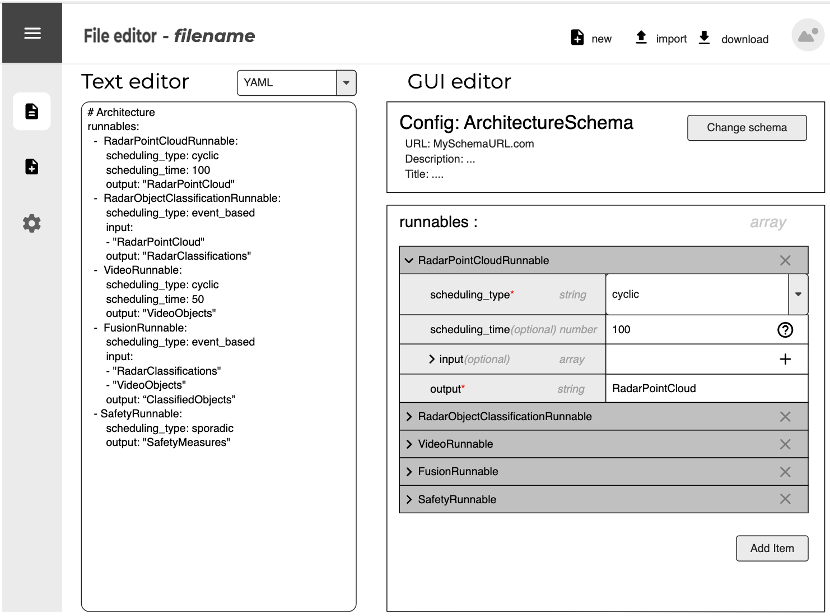
\includegraphics[width=\textwidth]{figures/mockup_gui_config}
    \caption{Sketch of the Tool before the implementation. File Editor view.}
    \label{mockup_gui_config}
\end{figure*}


\begin{figure*}[!thb]
    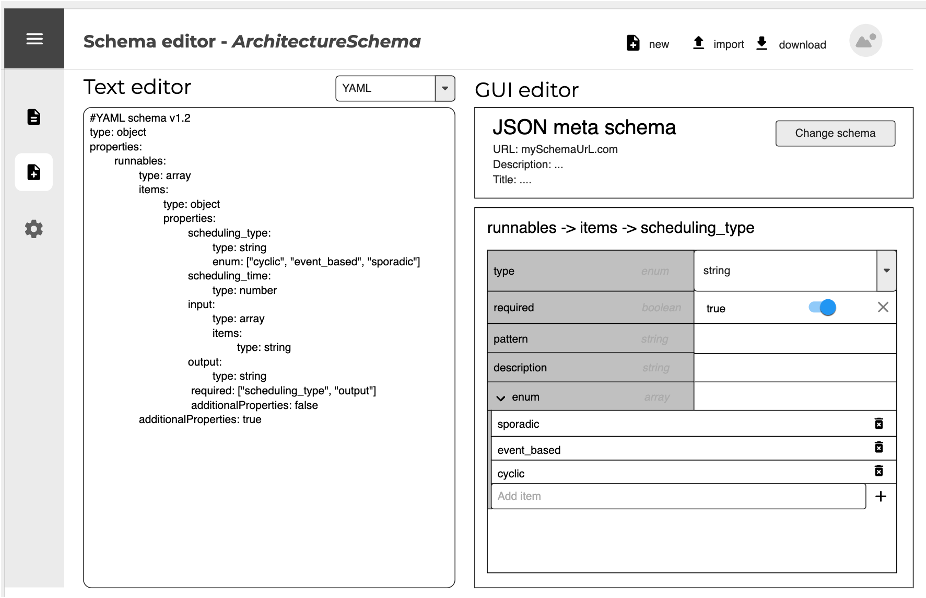
\includegraphics[width=\textwidth]{figures/mockup_gui_schema}
    \caption{Sketch of the Tool before the implementation. Schema Editor view.}
    \label{mockup_gui_schema}
\end{figure*}



\begin{figure*}[!htb]
    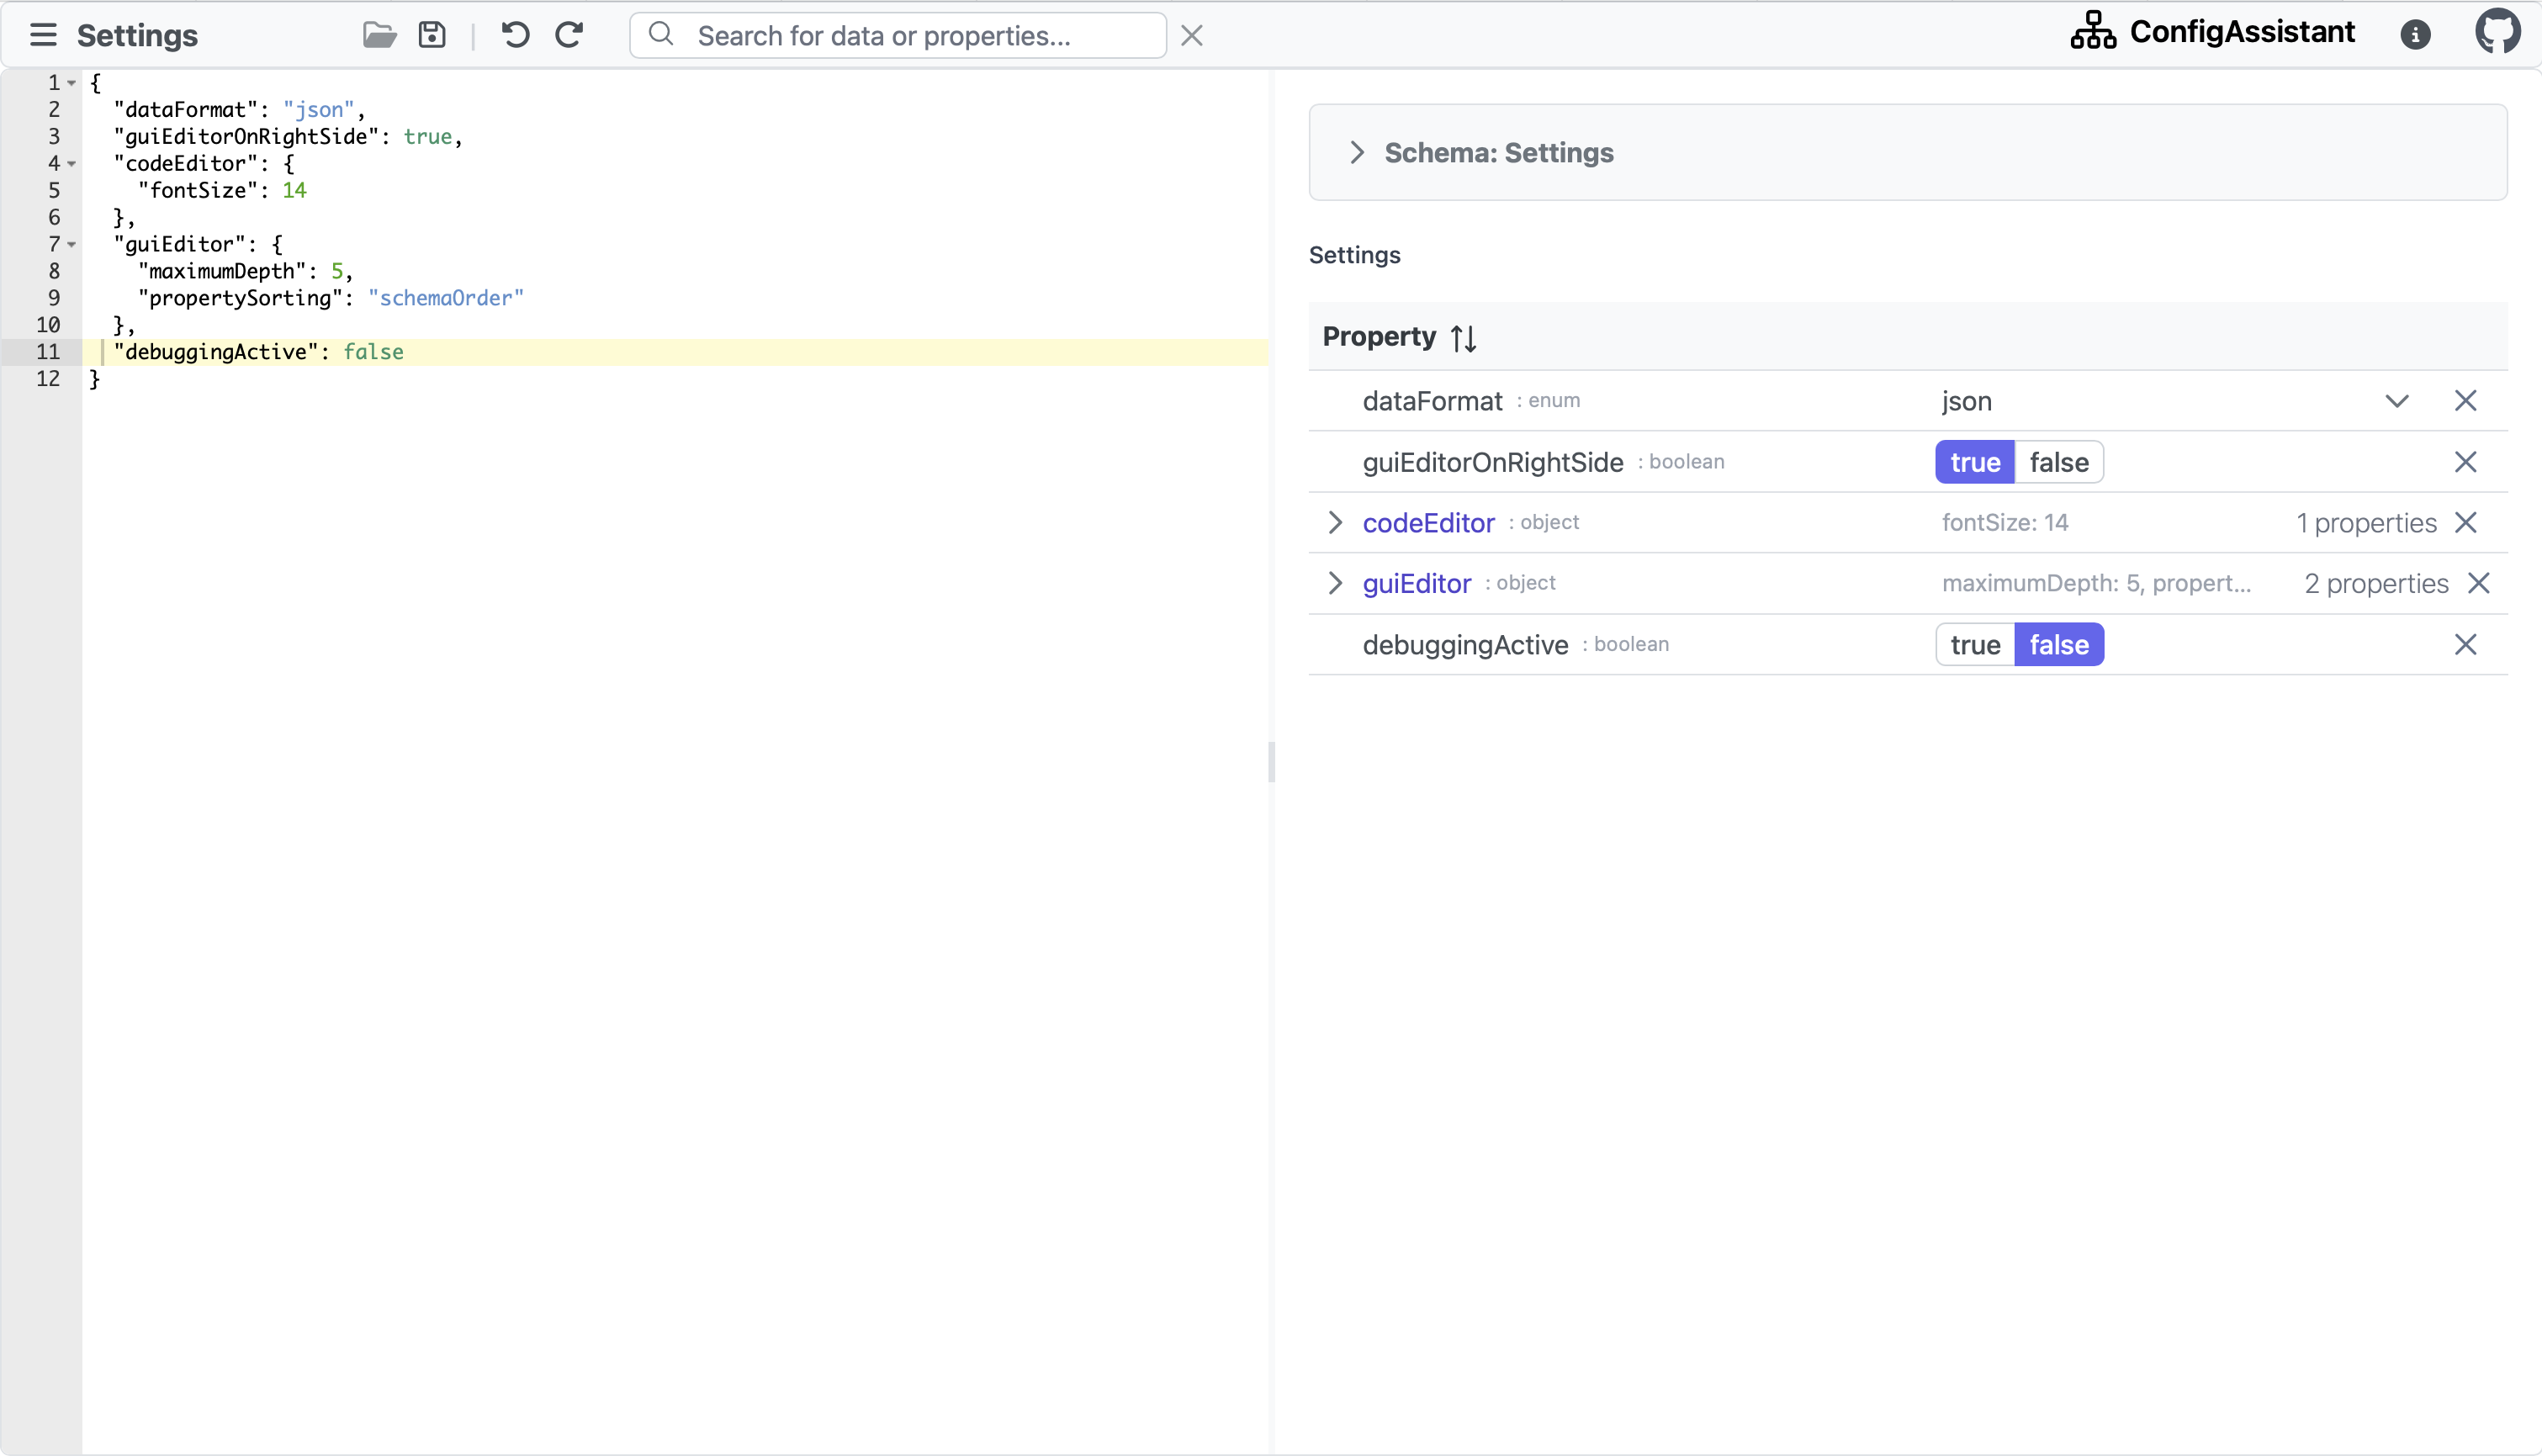
\includegraphics[width=\textwidth]{figures/settings}
    \caption{UI of Settings view}
    \label{fig:settings}
\end{figure*}



%\section{Implementation}\label{sec:appendix-implementation}
%\begin{table*}[!htb] % Use table* for wide tables
%    \caption{Libraries used in the implementation of our tool} %keyuri
%    \label{tab:libraries}
%    \centering
%    \begin{tabular}{ll}
%        \toprule
%        \textbf{Library} & \textbf{Purpose}     \\
%        \midrule
%        vue.js           & UI framework         \\
%        PrimeVue         & UI component library \\
%        Tailwind CSS     & CSS utility          \\
%        @fortawesome/fontawesome-svg-core & Font Awesome SVG icons. \\
%        ajv@8.12.0 & JSON schema validator for Node.js and browsers. \\
%        brace@0.11.1 & Browser-based code editor with syntax highlighting and code folding. \\
%        primeicons@6.0.1 & It is a popular UI component library for JavaServer Faces (JSF) applications. \\
%        \bottomrule
%    \end{tabular}
%\end{table*}


%\begin{table*}
%    \centering
%    \caption{Setting Parameters\label{tab:settings}}
%    \begin{tabular}{@{}p{0.3\linewidth}p{0.6\linewidth}@{}}
%        \toprule
%        \textbf{Parameter} & \textbf{\ Description} \\
%        \midrule
 %       Data Format & The data format used by the code editor. Currently YAML and JSON are supported. \\
 %       Code Editor Font Size & Size of the font in the code editor. \\
 %       Gui Editor On Right Side & By default, the GUI panel is located on the right side and the code panel on the left side. Using this option, their positions can be swapped. \\
%        GUI Editor Property Sorting & The order in which the properties in the GUI panel should appear:
%        \begin{itemize}
%            \item \textit{Schema Order}: Orders elements according to the order in the schema.
%            \item \textit{Priority Order}: Orders elements based on their priority (e.g. required properties first, deprecated %properties last).
%            \item \textit{Data Order }: Orders elements the same way as it is in the data.
%        \end{itemize} \\
%        GUI Editor Maximum Depth & Determines the maximum level of nesting or hierarchy displayed in the GUI editor. \\
%        Debugging Active & For debugging purposes, users can enable or disable the debugging panel as needed.  \\
%        \bottomrule
%    \end{tabular}
%\end{table*}


\section{User Study}\label{sec:user-study}  % Minye
\subsection{Interview Tasks}\label{subsec:tasks}
This part is about the newest version of interview tasks we prepared to conduct our user study.\\
\textbf{Remark:} Task 3 was added after the first user study and also some details in other tasks were modified.
\subsubsection{Introduction}
For these tasks you are presented a schema that you have not seen or worked with before.
We have prepared a schema of a made-up simulation software in which self-driving cars are simulated.
There is one self-driving car that has to navigate from a start point to an end point but there are also other vehicles and pedestrians simulated.
For these tasks, the exact details are not important.

\subsubsection{Task 1: Setup}
\begin{enumerate}
    \item Go to https://paulbredl.github.io/config-assistant/
    \item Select the option ``Select a Schema'': ``Example schema'', then ``Autonomous Vehicle Schema".
    \item Open the example configuration file we have sent to you. \\
          The following tasks will assume this schema and this example file.
\end{enumerate}

\subsubsection{Task 2: Questions}
\begin{enumerate}
    \item What is the name of the simulation?
    \item What is the weather in our simulated environment?
    \item What is the total duration of the simulation?
    \item Humidity is a subproperty of the Environment.
    Would 150 be a valid value for Humidity?
\end{enumerate}

\subsubsection{Task 3: Modifying the configuration file}
\begin{enumerate}
    \item Change the name of the simulation to Sim\_Advanced05.
    \item The VehicleType of the self-driving car is currently ``Level 3''.
    Change it to the highest possible level.
    \item The configuration file has validation errors, i.e., it is not valid according to the schema.
    \\ Find out what the errors are.
    Edit the file so it becomes a valid configuration.

\end{enumerate}

\subsubsection{Task 4: Modifying the schema}
\begin{enumerate}
    \item For many applications it is good practice or even required that a schema has a unique identifier, which usually is a URL.
          \\Set the \$id field of this schema to : ``https://www.example.com/self-driving-vehicle''.
    \item The simulation software will get a premium version in the next update, for which the user needs a license.
          The license key should be stored in the configuration file.
          Add a new property ``LicenseKey'' to the ``properties'' object.
          It should be of the type ``string''.
          The length of the key is at most 20 characters long.
    Add a short exemplary description.
    \item Go back to the file editor and verify that the new property ``LicenseKey'' is displayed and that the correct information is displayed when hovering over the property.
\end{enumerate}





% Minye

\subsection{User Study results}
\begin{table*}[!htbp]
    \centering
    \caption{Results of user study} \label{table:results}
    \begin{tabular}{lp{4.5cm}p{6cm}}
        \toprule
        &
        \thead{Accuracy \& Notes} & \thead{Difficulties} \\
        \midrule

        User Study 1 &
            Accuracy: 100\%(11/11)\newline
            Effective use of tooltips\newline
            Used both GUI and code editor

            &

            Task 3.2: Setting Vehicle Type to the highest level:\newline
            Took some time to find the field\\ \midrule

        User Study 2 &
            Accuracy: 91\%(10/11)\newline
            Used search functionality\newline
            Used both GUI and code editor

            &

            Task 4.2: Adding new property:\newline
            Could not find where to add new property in Schema Editor\newline
            Did not know how to edit property name \\ \midrule

        User Study 3 &
            Accuracy: 82\%(9/11)\newline
            Effective use of tooltips\newline
            Not familiar with JSON schema\newline
            Used only code editor in beginning and then only GUI editor after task 2.3.

            &

            Task 2.3: Duration of Simulation:\newline
            Did not think about using the GUI panel to retrieve information\newline
            Task 2.4: Validity of humidity:\newline
            Mistakenly thought humidity value was valid.\newline
            Did not consider red underline as an error\newline
            Task 4.2: Add new property:\newline
            Set property name in wrong place
         \\ \midrule

        User Study 4 &
            Accuracy: 82\%(9/11)\newline
            Solved tasks in a short time\newline
            Used only the GUI editor

            &

            Task 2.4: Validity of humidity:\newline
            Mistakenly thought humidity value was valid\newline
            Did not find out that he could use tooltips\newline
            Task 3.2: Setting Vehicle Type to the highest level: \newline
            Did not scroll down in Dropdown menu\newline
            Task 3.3: Validation Errors:\newline
            Thought red underline was spell checking \\ \midrule

        User Study 5 &
            Accuracy: 100\%(11/11)\newline
            Solved tasks in a short time\newline
            Used both GUI and code editor

            &

            Task 3.2: Setting Vehicle Type to the highest level: \newline
            Took some time to find the vehicle type \newline
            Task 4.2: Adding new property:\newline
        Did not set the property type at the beginning \\ \bottomrule
    \end{tabular}
\end{table*}


\begin{table*}[!htbp]
    \centering
    \caption{User Study 1 - Feedback and Solution}
    \label{tab:user_study1}
    \begin{tabular}{p{0.45\linewidth}p{0.45\linewidth}}
        \toprule
         \thead{Feedback} & \thead{Solution} \\
        \midrule
        The property value should not be autocorrected if the user enters an incorrect value.
        Instead, an error message or another way should be used to inform the user that their input is incorrect.
        &
        Instead of autocorrecting values, we now provide more clear user feedback on incorrect values (red underline, error symbol). \\
        \midrule
        It would be good to have the ability to remove data entries with the GUI panel.
        &
        Implemented by adding a \textit{remove} button next to properties which have data and are not required. \\
        \midrule
        A search functionality to locate properties would be helpful, especially within nested levels.
        & Implemented in the toolbar.
        All findings are highlighted in the GUI panel. \\
        \midrule
        %& 4. The Schema editor GUI panel contains extensive metadata, but the code editor panel remains empty. & 4. bla bla bla \\
        %\midrule
        The GUI panel feels overwhelming to the user due to many variations in styling and color of the GUI elements.
        &
        We slightly reduced the number of different styling by no longer showing required properties in bold face and instead just show an asterisk next to it. \\
        \midrule
        The cursor should not have the clickable animation when hovering over non-clickable fields in the GUI editor.
        &
        Now we only show the clickable animation when hovering over clickable GUI components. \\
        \midrule
        In drop-down menus we do not need a button to clear the selection.
        &
        We disabled the option of clearing the selection. \\
        \midrule
        If the type of a property is ``any'', it should not be interpreted as the ``string'' type in the GUI panel.
        &
        We show a drop-down menu to the user, where they can select the type they want to use. \\
        \midrule
        Validation errors should not be highlighted via a warning symbol, but instead an error symbol.
        &
        We changed the warning symbol into an error symbol. \\
        \midrule
        After performing an undo or redo action, the cursor should jump to the corresponding location to reflect the changes made by the user.
        &
        Will be considered in future work. \\
        \bottomrule
    \end{tabular}
\end{table*}


\begin{table*}

    \centering
    \caption{User Study 2 - Feedback and Solution}
    \label{tab:user_study2}
    \begin{tabular}{p{0.45\linewidth}p{0.45\linewidth}}
        \toprule
        \thead{Feedback} & \thead{Solution} \\
        \midrule
        A graph-based view would be more intuitive for handling complex data structures.
        &
        Will be considered in future work. \\
        \midrule
        Providing immediate feedback to users when they enter incorrect ranges is essential to prevent them from inputting invalid values into the property.
        &
        We now highlight schema violations by a red error symbol in the GUI panel and underlining the property name in red.
        Additionally, the tooltip lists all schema violations of a property. \\
        \midrule
        Validation errors should also be reflected in the GUI panel, including for child properties.
        &
        See point above.
        Also, now the tooltip lists schema violations of child properties. \\
        \midrule
        When dealing with an array, the display name of array elements (index) should be improved.
        Currently, the tool only shows just the element index.
        &
        We replaced the numerical labels by a standard programming notation, which is \texttt{propertyName[0]}, \texttt{propertyName[1]}, \ldots
        \\
        \midrule
        The input field next to the \textit{Add Item} button is confusing.
        Both the input field and the button can be used to create a new item, which is redundant.
        &
        We removed the input field next to the button. \\
        \midrule
        It would be more consistent, if all user input in the GUI panel was within the right column of the table.
        That in some scenarios user input is needed within the left column (for names of new properties) feels inconsistent.
        &
        Because of the nature of JSON schema, we retained the property name within the left column.
        To make it clear to the user that the property name can be edited, we added an \textit{edit} icon next to it. \\
        \midrule
        The search function for locating specific properties lacks clarity at first glance.
        It should provide an immediate response and extend to nested levels, rather than merely highlighting the higher-level findings.
        &
        The search now provides a list of results, and upon clicking on a particular result, it jumps to that result in the code panel and GUI panel.
        In the GUI panel, if the element is nested, its parents will be automatically expanded. \\
        \bottomrule
    \end{tabular}

\end{table*}

\begin{table*}
    \centering
    \caption{User Study 3 - Feedback and Solution} \label{tab:user_study3}
    \begin{tabular}{p{0.45\linewidth}p{0.45\linewidth}}
        \toprule
        \thead{Feedback} & \thead{Solution} \\
        \midrule
        Working with the schema editor is difficult for me.
        It does not feel intuitive.
        &
        We made the schema editor more intuitive by creating our own simplified JSON schema meta schema.
        For example, advanced JSON schema features are separated from the simple ones.
        See section~\ref{subsec:schema-editor} \\
        \bottomrule

    \end{tabular}

\end{table*}

\begin{table*}
    \centering
    \caption{User Study 4 - Feedback and Solution} \label{tab:user_study4}
    \begin{tabular}{p{0.45\linewidth}p{0.45\linewidth}}
        \toprule
        \thead{Feedback} & \thead{Solution} \\
        \midrule
        Modifying or renaming a new property in the GUI panel does not appear to take effect when double-clicking on it.
        &
        Renaming properties in the GUI panel can now be done using the \textit{edit} button next to the property name. \\
        \midrule
        When creating a new property in the schema editor, its sub-schema has to be selected, such as \textit{string property} or \textit{boolean property}.
        Additionally, the type of the property has to be selected by the user too.
        Therefore, for example, when creating a new \textit{string property}, the user has to select that it is a string two times.
        It would be much more intuitive if the selection needs to be done only one time.
        & We completely overhauled our JSON schema meta schema.
        Now, when creating a new property, the user will have to select the type only once. \\
        \midrule
        A toggle button should be implemented to enable and disable the code panel and GUI panel.
        & Only having a GUI panel or only having a code panel restricts the user unnecessarily.
        The interplay of both panels is what makes this tool most effective.
         If the user does not want to use one of the panels, they can resize that panel to a very small size.  \\
        \midrule
        When working with a particular property in the GUI panel the opacity of the other properties should be decreased, visually highlighting the property that currently is in focus. & Will be considered in future work. \\
        \midrule
        Simplify the schema editor to make it easier to work with, for those who are not very familiar with JSON schema.
        &
        Has been done, see section~\ref{subsec:schema-editor}. \\
        \bottomrule

    \end{tabular}

\end{table*}

\begin{table*}

    \centering
    \caption{User Study 5 - Feedback and Solution} \label{tab:user_study5}
    \begin{tabular}{p{0.45\linewidth}p{0.45\linewidth}}
        \toprule
        \thead{Feedback} & \thead{Solution} \\
        \midrule
        The search button is not immediately evident, making it challenging for users to locate the search function. &
        Instead of showing the search bar only when clicking the search button, we now always show it. \\
        \bottomrule

    \end{tabular}

\end{table*}




%
% \vspace{11pt}
%
% \textbf{If you include a photo:}\vspace{-33pt}
%\begin{IEEEbiography}%[{\includegraphics[width=1in,height=1.25in,clip,keepaspectratio]{fig1}}]{Michael %Shell}
%Use $\backslash${\tt{begin\{IEEEbiography\}}} and then for the 1st argument use %$\backslash${\tt{includegraphics}} to declare and link the author photo.
%Use the author name as the 3rd argument followed by the biography text.
%\end{IEEEbiography}

%
% \textbf{If you will not include a photo:}\vspace{-33pt}
% \begin{IEEEbiographynophoto}{John Doe}
%  Use $\backslash${\texttt{begin\{IEEEbiographynophoto\}}} and the author name as the argument followed by the biography text.
% \end{IEEEbiographynophoto}


\end{document}


